%%%%%%%%%%%%%%%%%%%%%%%%%%%%%%%%%% MAIN SETTINGS %%%%%%%%%%%%%%%%%%%%%%%%%%%%%%%%%%%%%%%%

\documentclass[
LEEC,			% Use this option to select your DEE degree, options: LEEC, LETI
english,		% Select document language, options: portuguese or english
%draft,	% Uncomment for draft mode (no pictures, no links, overfull hboxes) 
%twocolumn
]{DEEclass}

% Use the 'preamble.tex' file (root folder) do add packages and macros. Keep your main.tex file clean.

% FYI, the following packages are preloaded with the document class:
% longtable, xcolor, graphicx, booktabs, caption, csquotes, hyperref,
% calc, listings, datetime2, siunitx, geometry, enumitem

%%%%%%%%%%%%%%%%%%%%%%%%%%%%%%%%%%%%%%%%%%%%%%%%%%%%%%%%%% extra packages
\usepackage{amsmath}		% the main package in the AMS-LATEX distribution
\usepackage{amsfonts}		% extended set of fonts for use in mathematics
\usepackage{amssymb}		% adds new symbols to be used in math mode
\usepackage{mathrsfs}		% math fonts, e.g., Laplace
\usepackage{float}			% provides the H float modifier option
\usepackage{multirow}		% tables \multirow command
\usepackage{subcaption}		% enables subfigures
\usepackage{lscape}			% for landscape mode
\usepackage{verbatim}		% new verbatim environment, 
\usepackage{multicol}		% enables multicolumns 
\usepackage[intoc, english]{nomencl} % add nomenclature
\makenomenclature
\usepackage{etoolbox}       % used for nomenclature, i guess...
\makeglossaries
\usepackage{wrapfig}        % enable wrapping figures graphics
\usepackage{graphicx}       % enable graphics
\let\cleardoublepage=\clearpage     % delete blank pages
%\begin{comment}...\end{comment}, \verbatiminput


%add extra packages if needed here

%%%%%%%%%%%%%%%%%%%%%%%%%%%%%%%%%%%%%%%%%%%%%%%%%%%%%%%%%% temp packages
\usepackage{lipsum}						% for fake text
%\usepackage[textsize=tiny]{todonotes}   % enable To-do notes, use the option "disable" to hide all notes, usage \todo{}

%\usepackage{draftwatermark}			% prints a watermark overlay, uncomment if needed
%\SetWatermarkText{**DRAFT**}
%\SetWatermarkScale{1}
%\SetWatermarkColor[gray]{0.8}

%%%%%%%%%%%%%%%%%%%%%%%%%%%%%%%%%%%%%%%%%%%%%%%%%%%%%%%%%% settings
\AtBeginDocument{					% Rendered PDF metadata:
\hypersetup{pdftitle=\ttitle} 		% Sets the PDF title to your dissertation title
\hypersetup{pdfauthor=\authorname} 	% Sets the PDF author to your name
}

%%%%%%%%%%%%%%%%%%%%%%%%%%%%%%%%%%%%%%%%%%%%%%%%%%%%%%%%%% user defined macros









	
% \makenomenclature

%%%%%%%%%%%%%%%%%%%%%%%%%%%%%%%% REPORT INFORMATION %%%%%%%%%%%%%%%%%%%%%%%%%%%%%%%%%%%%%

\reporttitle{Designing the new Ozone kite for the 2028 Olympic Games} % Your report title

\author{Romain Lambert}	% Your name
\studentnumber{0673627662}	% Your student number
\studentemail{1234567@isep.ipp.pt}	% Your student email address  

\advisor{Nome do Orientador}{xxx@isep.ipp.pt}	% Your ISEP advisor name and email
\coadvisor{Nome do Coorientador}{xxx@isep.ipp.pt}	% Your ISEP co-advisor name and email, comment this line if not needed
\company{Nome da Empresa, Lda.}	% The company name where you developed your work, comment this line if not needed
\supervisor{Nome do Orientador da Empresa}{xxx@emailaddress.com} % Your company supervisor name, comment this line if not needed

%%%%%%%%%%%%%%%%%%%%%%%%%%%%%%%%%%%%%%%%%%%%%%%%%%%%%%%%%%%%%%%%%%%%%%%%%%%%%%%%%%%%%%%%%
\begin{document}

\pagestyle{plain} % Default to the plain heading style until the thesis style is called for the body content

\printcoverpage

%%%%%%%%%%%%%%%%%%%%%%%%%%%%%%%%%%% FRONTMATTER %%%%%%%%%%%%%%%%%%%%%%%%%%%%%%%%%%%%%%%%%
% Consider the following front matter sections provided as separate files in the 'front' folder.
% Comment the lines regarding the sections you will not use, or edit the file contents as needed

\tableofcontents

\listoffigures
%% This code creates the groups
% -----------------------------------------
\renewcommand\nomgroup[1]{%
  \item[\bfseries
  \ifstrequal{#1}{C}{Computational fluid dynamics}{%
  \ifstrequal{#1}{K}{Kite flight modelling}{%
  \ifstrequal{#1}{S}{Sailing vocabulary}{}}}%
]}
% -----------------------------------------

\nomenclature[C]{\(\textbf{CFD}\)}{Computational fluid dynamics}
\nomenclature[C]{\(\textbf{VLM}\)}{Vortex lattice method}

\nomenclature[k]{\(\textbf{V$_{WR}$}\)}{Relative wind velocity at kite altitude}
\nomenclature[k]{\(\textbf{V$_{WT}$}\)}{True wind velocity}
\nomenclature[k]{\(\textbf{V$_{s}$}\)}{Ship velocity}
\nomenclature[k]{\(\textbf{$\alpha_{i}$}\)}{Kite angle of attack}
\nomenclature[k]{\(\textbf{$\delta$}\)}{Angle between the athlete and his lines}
\nomenclature[k]{\(\textbf{V$_{a}$}\)}{Apparent wind velocity seen by the kite}
\nomenclature[k]{\(\textbf{V$_{k}$}\)}{Kite velocity}
\nomenclature[k]{\(\textbf{F$_{a}$}\)}{Aerodynamic resultant}
\nomenclature[k]{\(\textbf{T}\)}{Tethers tension}
\nomenclature[k]{\(\textbf{$\alpha_{S, WT}$}\)}{Angle between the rider and the true wind speed}
\nomenclature[k]{\(\textbf{$\epsilon$}\)}{Angle between the kite's velocity vector and the apparent wind}
\nomenclature[k]{\(\textbf{$\alpha_{a,WT}$}\)}{Angle between the apparent wind speed and the true wind speed}

\nomenclature[S]{\(\textbf{VMG}\)}{Velocity Made Good}
\printnomenclature

%\include{front/2_acknowledgements}	% Edit to add the due acknowledgements, or comment this line if not used
%\include{front/3_abstract}			% Edit the file to write the document Abstract. Two languages are always required.
%\include{front/4_frontmatterlists}	% Edit the file to select the lists to be shown (figures, tables, source code segments, glossary, acronyms, symbols)

%%%%%%%%%%%%%%%%%%%%%%%%%%%%%%%%%%% MAINMATTER %%%%%%%%%%%%%%%%%%%%%%%%%%%%%%%%%%%%%%%%%

% Include the chapters of the document as separate files from the 'chapters' folder

\include{chapters/Introduction}
%%%%%%%%%%%%%%%%%%%%%%%%%%%%%%%%%%%% Chapter Template

\chapter{2D steady simulations} 	% Main chapter title
\label{Chapter1} 		% For referencing the chapter elsewhere, usage \ref{Chapter1}

%%%%%%%%%%%%%%%%%%%%%%%%%%%%%%%%%%%%

The initial goal was to identify the factors that contribute to the VMG's superior efficiency compared to the R1V4 and make the necessary adjustments.

The first step involved identifying the parameters that respond to various flight conditions. Following that, a low-fidelity approach using XFLR5 was employed to compute the 2D aerodynamic coefficients, providing insights into the disparities between the airfoils. Subsequently, Fluent CFD software was utilized to obtain a more precise assessment of the aerodynamic coefficients for each airfoil during actual flight conditions.

%%%%%%%%%%%%%%%%%%%%%%%%%%%%%%%%%%%%%%%%%%%%%%%%%%%%%%%%%%%%%%%%%%%%%%%%%%%%%%%%
%%%%%%%%%%%%%%%%%%%%%%%%%%%%%%%%%%%% SECTION 1 %%%%%%%%%%%%%%%%%%%%%%%%%%%%%%%%%
%%%%%%%%%%%%%%%%%%%%%%%%%%%%%%%%%%%%%%%%%%%%%%%%%%%%%%%%%%%%%%%%%%%%%%%%%%%%%%%%

\section{Kite flight modelling}
\label{sec:Ch1.1}

The kite is modelized according to the "zero mass model" as developed in the course given by Richard Leloup in Supaero \cite{cours_leloup}.

\begin{figure}[H]
    \centering
    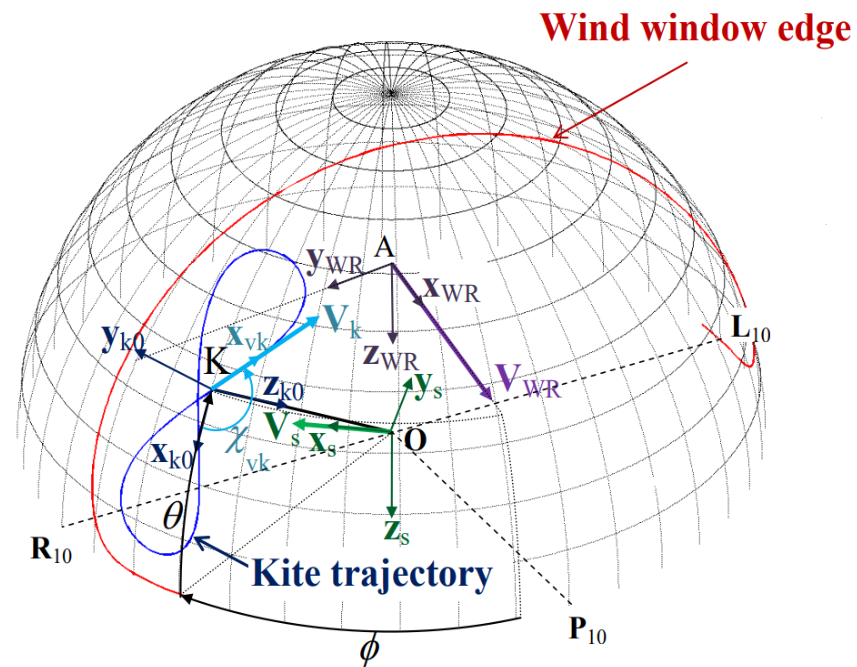
\includegraphics[width=0.7\textwidth]{figures/2D steady simulations/kite flight modeling 1.png}
    \caption{Speeds \& angles decomposition}
    \label{fig:Kite_flight_modelling}
\end{figure}

\begin{figure}[H]
    \centering
    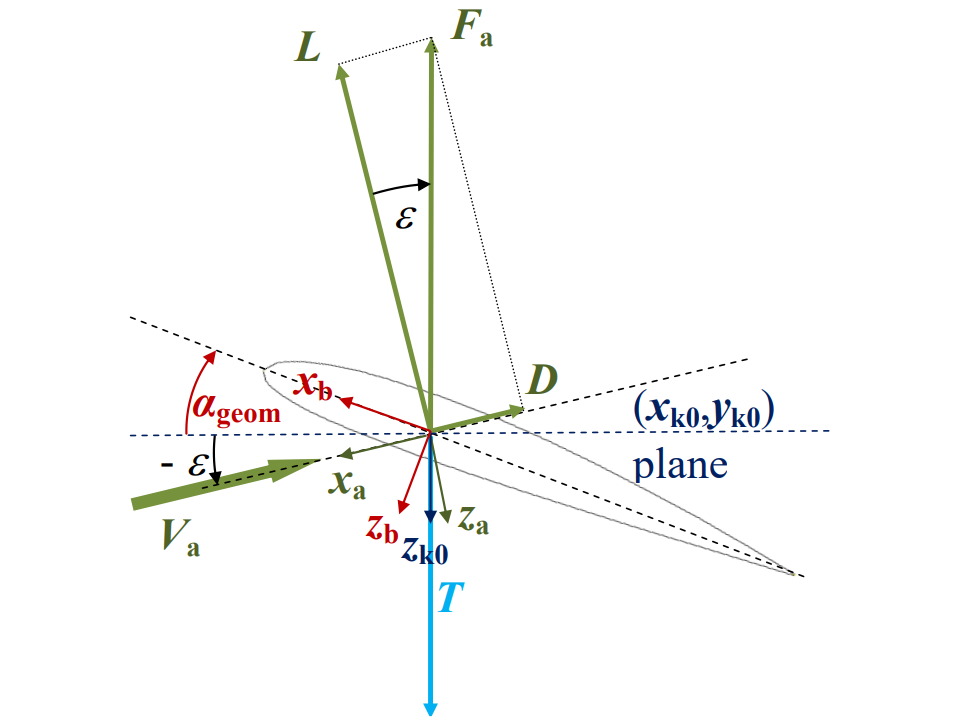
\includegraphics[width=0.8\textwidth]{figures/2D steady simulations/kite flight modeling 2.png}
    \caption{Decomposition of the aerodynamic force vector}
    \label{fig:Kite_flight_modelling}
\end{figure}

The Zero-mass model approach leads to the following results : 
\begin{equation}
\left \{
   \begin{array}{r c l}
      V_{WR}  & = & V_{WT} - V_{S} \\
      V_{a}   & = & V_{WR} - V_{k} \\
      F_{a} & = & -T = \frac{1}{2}\frac{C_{L} \rho A V_{a}^{2}}{cos(\epsilon)}
   \end{array}
   \right .
   \label{kite_speed_vectors}
\end{equation}

with, in our case of study, $V_{k} = 0$. As a matter of fact, we are assuming that the kite is static in relation to the ship (the rider). 


Then, we can deduce from the relation \ref{kite_speed_vectors} : 
\begin{equation}
\left \{
   \begin{array}{r c l}
      V_{a}  & = & \sqrt{V_{WT}^2 + V_{S}^2 - 2V_{WT}V_{S}cos(\alpha_{S, WT}) } \\
      \epsilon   & = & \alpha_{S, WT} - \alpha_{a, WT} \\
      \alpha_{a, WT} & = & arctan(\frac{V_{s}sin(\alpha_{S, WT})}{V_{s}cos(\alpha_{S, WT}) - V_{WT}})
   \end{array}
   \right .
   \label{kite_speed_vectors_2}
\end{equation}


\begin{wrapfigure}{r}{0.6\textwidth}
\centering
    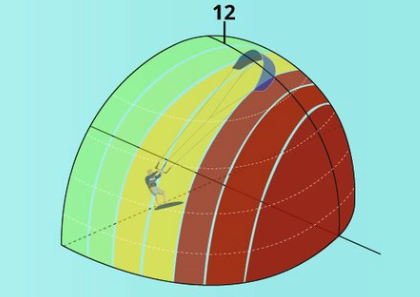
\includegraphics[width=0.5\textwidth]{figures/2D steady simulations/kite flight modeling 3.png}
    \caption{The wind window}
    \label{fig:The_wind_window}
\end{wrapfigure}

Then, we understand that depending on the position of the kite ($\Phi, \Theta$), the rider's speed ($V_{s}$) and the true wind speed ($V_{WT}$), the tether tension (T) is very different. This result has lead to the definition of the wind window represented on the figure \ref{fig:The_wind_window}.

The concept of the wind window holds significant importance in kitesurfing as it presents riders with a fundamental trade-off: the closer the kite is positioned to the center of the wind window, the more power it generates. However, this ideal kite placement might not align with the rider's intended direction. As a result, kitesurfers must strategically position their kites within the wind window to maximize power in their desired direction.


%%%%%%%%%%%%%%%%%%%%%%%%%%%%%%%%%%%%%%%%%%%%%%%%%%%%%%%%%%%%%%%%%%%%%%%%%%%%%%%%
%%%%%%%%%%%%%%%%%%%%%%%%%%%%%%%%%%%% SECTION 2 %%%%%%%%%%%%%%%%%%%%%%%%%%%%%%%%%
%%%%%%%%%%%%%%%%%%%%%%%%%%%%%%%%%%%%%%%%%%%%%%%%%%%%%%%%%%%%%%%%%%%%%%%%%%%%%%%%
\section{The different phases}
\label{sec:Ch1.3}

A kite race is segmented into distinct phases, each corresponding to varying inlet conditions. What's of primary importance for the riders during these phases is their "Velocity Made Good," often referred to as VMG, which signifies their speed aligned with the axis they intend to follow (the wind axis).

\begin{figure}[H]
    \centering
    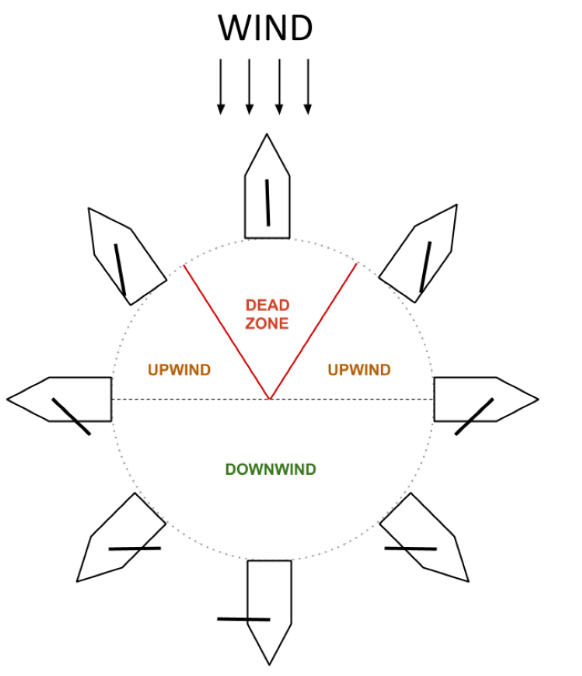
\includegraphics[width=0.5\textwidth]{figures/2D steady simulations/upwind_downwind_scheme.png}
    \caption{Upwind and downwind diagram}
    \label{fig:upwind_downwind_scheme}
\end{figure}

%%%%%%%%%%%%%%%%%%%%%%%%%%%%%%%%%%%% SUBSECTION 1

\subsection{The upwind}
\label{sub:Ch1.3.1}

Advancing upwind involves traveling in the direction opposite to the wind. This segment typically accounts for approximately $\frac{2}{5}$ of the entire race. 

In this phase, the kite operates at lower angles of attack, resulting in its highest relative speed. Riders in this phase aim to strike a balance between gripping the bar for increased power, which can cause the kite to shift back within the wind window, and releasing the bar for reduced tether tension, allowing the kite to move toward the edge of the wind window.

%%%%%%%%%%%%%%%%%%%%%%%%%%%%%%%%%%%% SUBSECTION 2

\subsection{The downwind}
\label{sub:Ch1.3.1}

Heading downwind involves traveling in the same direction as the wind. This phase typically constitutes about $\frac{2}{5}$ of the entire race duration. In this stage, the kite operates with steep angles of attack, resulting in its slowest relative speed.

As a consequence, the rider must maintain a firmer grip on the bar to increase their VMG (enabling them to head as far downwind as possible). However, they also need to release the bar at times, allowing the kite to move freely, in order to increase tether tension – the opposite of what's done during the upwind phase. In this phase, maintaining tension in the lines proves to be particularly challenging due to the slower relative speed. Additionally, a larger kite provides the rider with more power during this phase.

%%%%%%%%%%%%%%%%%%%%%%%%%%%%%%%%%%%% SUBSECTION 3

\subsection{The transition}
\label{sub:Ch1.3.1}

The transition is the moment when the rider changes direction (tacks or jibes). At this moment, the rider doesn't want the kite to lift him out of the water, or he would loose his balance and fall. 

%%%%%%%%%%%%%%%%%%%%%%%%%%%%%%%%%%%% SUBSECTION 4

\subsection{The crosswind}
\label{sub:Ch1.3.1}

This phase represents around $\frac{1}{5}$ of the entire race. It has not been considered in this study as it relies on the upwind and downwind performances. 

%%%%%%%%%%%%%%%%%%%%%%%%%%%%%%%%%%%%%%%%%%%%%%%%%%%%%%%%%%%%%%%%%%%%%%%%%%%%%%%%
%%%%%%%%%%%%%%%%%%%%%%%%%%%%%%%%%%%% SECTION 3 %%%%%%%%%%%%%%%%%%%%%%%%%%%%%%%%%
%%%%%%%%%%%%%%%%%%%%%%%%%%%%%%%%%%%%%%%%%%%%%%%%%%%%%%%%%%%%%%%%%%%%%%%%%%%%%%%%

\section{Experimental data }
\label{sec:Ch1.2}

Ozone benefits from working with world-renowned kiters, also known as "team riders". Axel Mazella, two times Kitefoil World Champion (2017 and 2019) and European Champion (2019), is a racing team rider and tester for Ozone. Thanks to him, I have had access to his Palma racing (29/04/2023) data that are a "good reference" for understanding speeds and angles that are to be considered in a formula kite race.  

The following table \ref{tab:Average_data_from_Axels_race} gives the average values from this very race : 

\begin{table}[H]
    \center
    \begin{tabular}{|l|l|l|l|}
        \hline
            & $\alpha_{s, WT} ($°$) $ & $V_{WT} (knots) $ & $V_{S} (knots) $ \tabularnewline
        \hline
        Upwind & 39,5 & 14,0 & 22,5  \tabularnewline
        \hline
        Downwind & 155,0 & 14,0 & 31,5  \tabularnewline
        \hline
    \end{tabular}
    \caption{Average data from Axel's race}
    \label{tab:Average_data_from_Axels_race}
\end{table}

From these values and according to the equation \ref{kite_speed_vectors_2}, we can deduce (\ref{tab:Average_data_from_Axel's_race_2}): 

\begin{table}[H]
    \center
    \begin{tabular}{|l|l|l|}
        \hline
             & $\epsilon ($°$) $ & $V_{a} (knots) $ \tabularnewline
        \hline
        Upwind & 15,0 & 34,5  \tabularnewline
        \hline  
        Downwind & 15,0 & 20,5  \tabularnewline
        \hline
    \end{tabular}
    \caption{Average $\epsilon$ and $V_{a}$ from Axel's race}
    \label{tab:Average_data_from_Axel's_race_2}
\end{table}

Nonetheless, these $\epsilon$ values appear impractical as they would imply angles of attack exceeding 15°, which is excessively high.

Conversations with the Ozone team and other kitesurfing experts, including individuals like Benoît Augier, a researcher specializing in fluid mechanics at the Marine Hydrodynamics Laboratory in Brest, who closely collaborates with the French Kitesurfing team for the Olympic Games, revealed that these $\epsilon$ values are notably distant from reality. In fact, they represent a realm of calculations that has yet to be theoretically determined and prove challenging to measure through experimental means.

As a matter of fact, The previous results assume a 90° angle between the rider and his lines. However, as shown in \ref{new angles}, the position of the kite in the wind window and the position of the bar (handled by the rider) constantly change while kitesurfing and greatly modify the value of $\alpha_{i}$. Moreover, the link between the lift and the tether tension from \ref{kite_speed_vectors} is changed if we considered the lines to make an angle $\delta$ with the athlete.

Nevertheless, considering the physical limitations and the aerodynamic flight equations of a kite, it is possible to derive the following outcomes :

\begin{equation}
\left \{
   \begin{array}{r c l}
      \delta  & \in & [0, \epsilon] \\
      Tcos(\delta)   & = & Lcos(\epsilon) \\
      a_{geom} + \epsilon - \delta & = & \alpha_{i}
   \end{array}
   \right .
   \label{new angles}
\end{equation}

\begin{figure}[H]
    \centering
    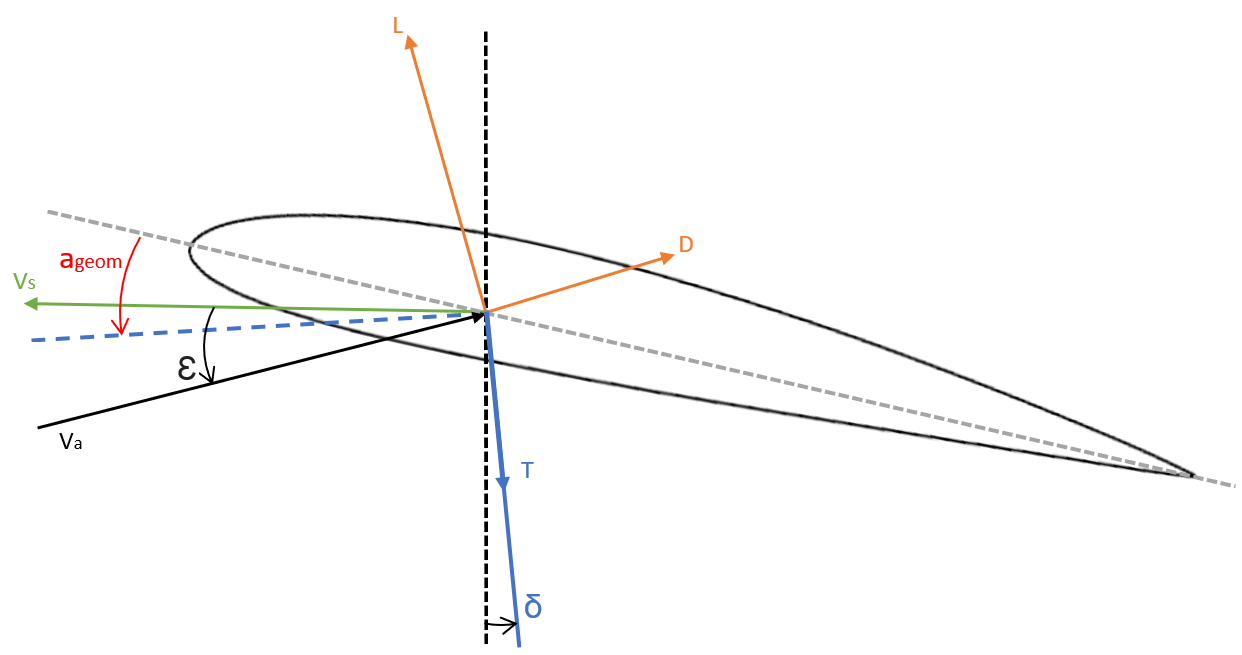
\includegraphics[width=1\textwidth]{figures/2D steady simulations/Angle calcul.png}
    \caption{Angle decomposition, taking into account the angle $\delta$ between the lines and the athlete}
    \label{fig:Angle decomposition, taking into account the angle $\delta$ between the lines and the athlete}
\end{figure}

\begin{figure}[H]
    \centering
    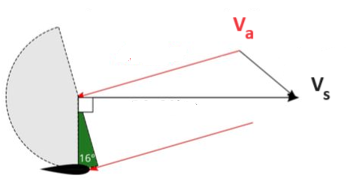
\includegraphics[width=0.6\textwidth]{figures/2D steady simulations/Ifremer work.png}
    \caption{The range of possible values for $\delta$ with an angle between the athlete's velocity vector and the apparent wind of 16°}
    \label{fig:The range of possible values for epsilon for an angle between the athlete's velocity vector and the apparent wind of 16°}
\end{figure}

 Consequently, the table \ref{tab:commonly_accepted_inlet_values} presents the generally acknowledged input parameters for a kite, as per the insights of kitesurfing experts and in consideration of Axel's race data :

 \begin{table}[H]
    \center
    \begin{tabular}{|l|l|l|}
        \hline
             & $\alpha_{i} ($°$) $ & $V_{a} (knots) $ \tabularnewline
        \hline
        Upwind & 0 - 5 & 30 - 35  \tabularnewline
        \hline
        Downwind & 7 - 14 & 18 - 23  \tabularnewline
        \hline
    \end{tabular}
    \caption{Commonly accepted inlet values}
    \label{tab:commonly_accepted_inlet_values}
\end{table}

%%%%%%%%%%%%%%%%%%%%%%%%%%%%%%%%%%%%%%%%%%%%%%%%%%%%%%%%%%%%%%%%%%%%%%%%%%%%%%%%
%%%%%%%%%%%%%%%%%%%%%%%%%%%%%%%%%%%% SECTION 4 %%%%%%%%%%%%%%%%%%%%%%%%%%%%%%%%%
%%%%%%%%%%%%%%%%%%%%%%%%%%%%%%%%%%%%%%%%%%%%%%%%%%%%%%%%%%%%%%%%%%%%%%%%%%%%%%%%

\section{XFLR5 - The plot of the aerodynamic polars}
\label{sec:Ch1.4}

%%%%%%%%%%%%%%%%%%%%%%%%%%%%%%%%%%%% SUBSECTION 1

\subsection{XFLR5}
\label{sub:Ch1.4.1}

XFLR5 is an analysis tool for airfoils, wings and planes operating at low Reynolds Numbers.

\begin{figure}[H]
    \centering
    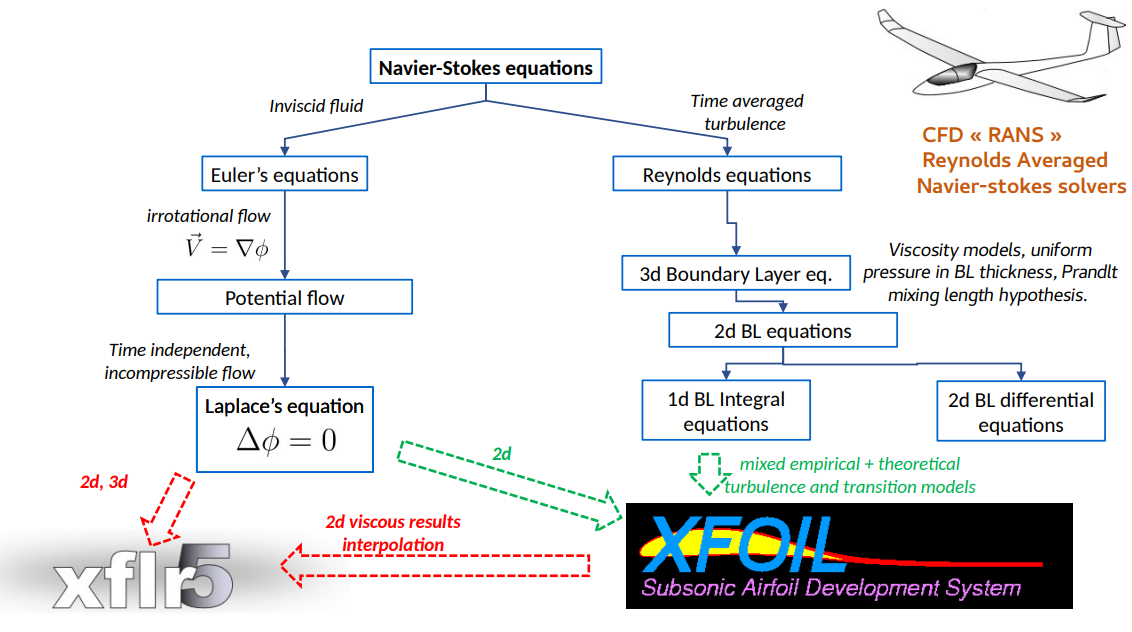
\includegraphics[width=1\linewidth]{figures/2D steady simulations/XFLR5 theory.png}
    \caption{XFLR5 theory diagram}
    \label{fig:XFLR5_theory_diagram}
\end{figure}

XFLR5 uses the "simultaneous" scheme, Developed by M. Drela and H. Youngren in the 1990s (XFOIL) at MIT, for solving the interactive boundary layer problem. It means that the inviscid and boundary layer equations are solved concurrently at each iteration\cite{XFLR5doc}.

In 2d, XFoil implements a full interactive boundary layer loop. However, XFOIL ultimately yields results that are accurate within the linear angle of attack range and below a Mach number of 0.4 but tends to overpredict lift and underpredict drag unless the flow is in the compressible regime. XFOIL cannot accurately model stall and post-stall conditions due to the nature of the solver\cite{XFOILlimits}.

%%%%%%%%%%%%%%%%%%%%%%%%%%%%%%%%%%%% SUBSECTION 2

\subsection{The polars}
\label{sub:Ch1.4.2}

Using XFLR5, I was able to plot the polars of the "R1 V4", the current Ozone kite, the "R1 V5", the next version of the R1 kites and the "VMG", the current kite of Flysurfer that was to be outperformed. 

The upwind polars have been plotted using a speed of 35 knots and a Reynolds number of $1,3e^{6}$

\begin{figure}[H]
\begin{subfigure}{0.5\textwidth}
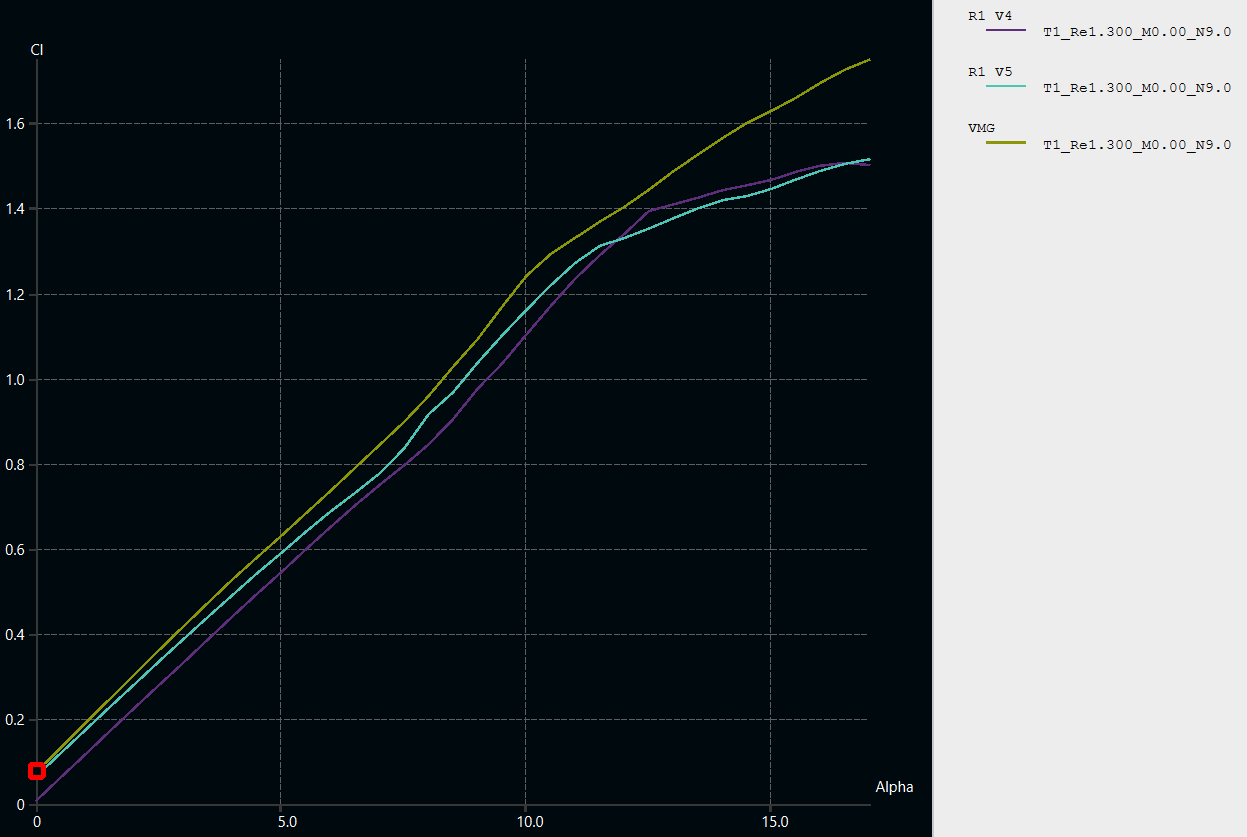
\includegraphics[width=1.\textwidth]{figures/2D steady simulations/xflr5/Cl upwind.png}
\caption{Plot of Cl upwind}
\label{fig:Plot_of_Cl_upwind}
\end{subfigure}
\begin{subfigure}{0.5\textwidth}
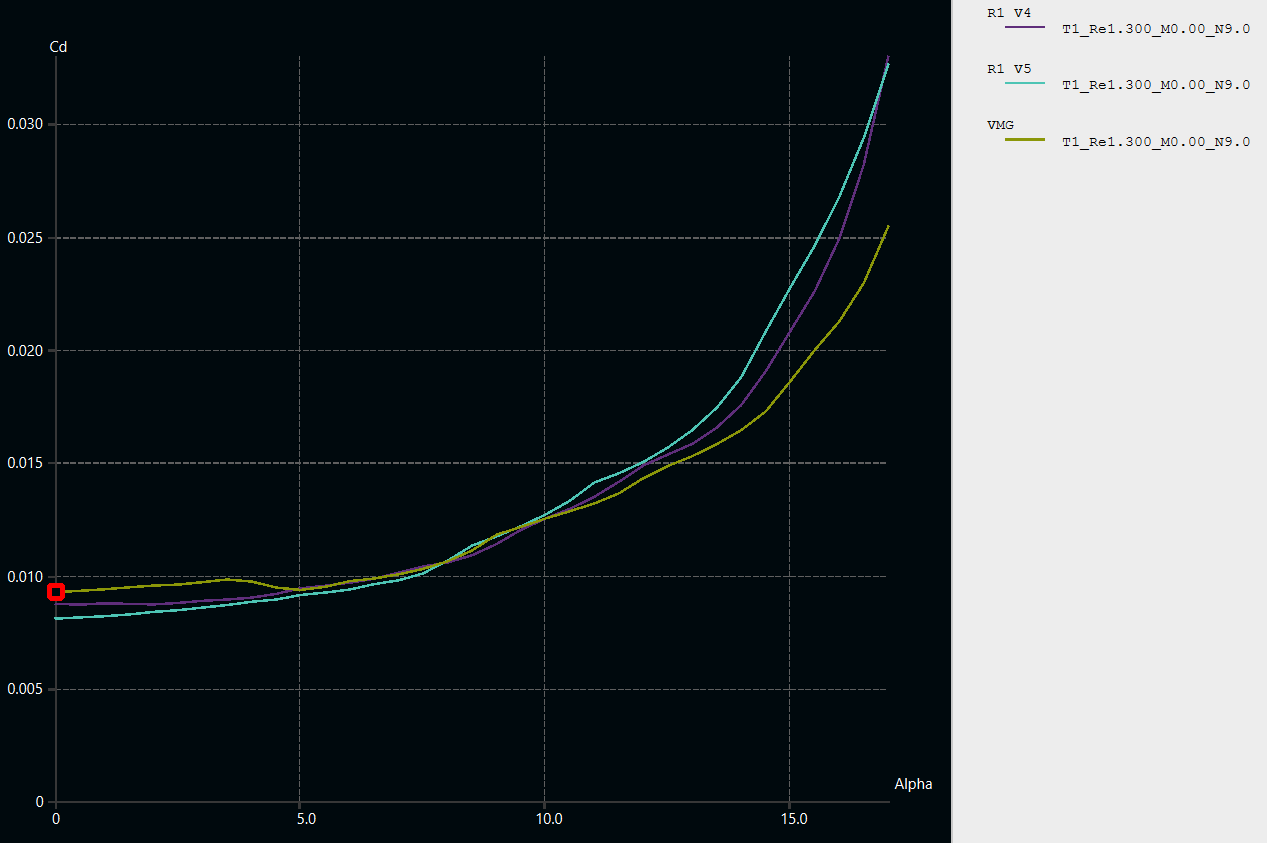
\includegraphics[width=01.\textwidth]{figures/2D steady simulations/xflr5/Cd upwind.png}
\caption{Plot of Cd upwind}
\label{fig:Plot_of_Cd_upwind}
\end{subfigure}
\caption{Upwind plots}
\label{fig:Upwind_plots}
\end{figure}

These polars are interesting for low angles of attack ( 0-5° according to \ref{tab:commonly_accepted_inlet_values} ) where one can see that the VMG and R1 V5 have a higher Cl than the R1 V4 and the R1 V5 has a lower Cd than the R1 V4 and the VMG. 

\begin{figure}[H]
    \centering
    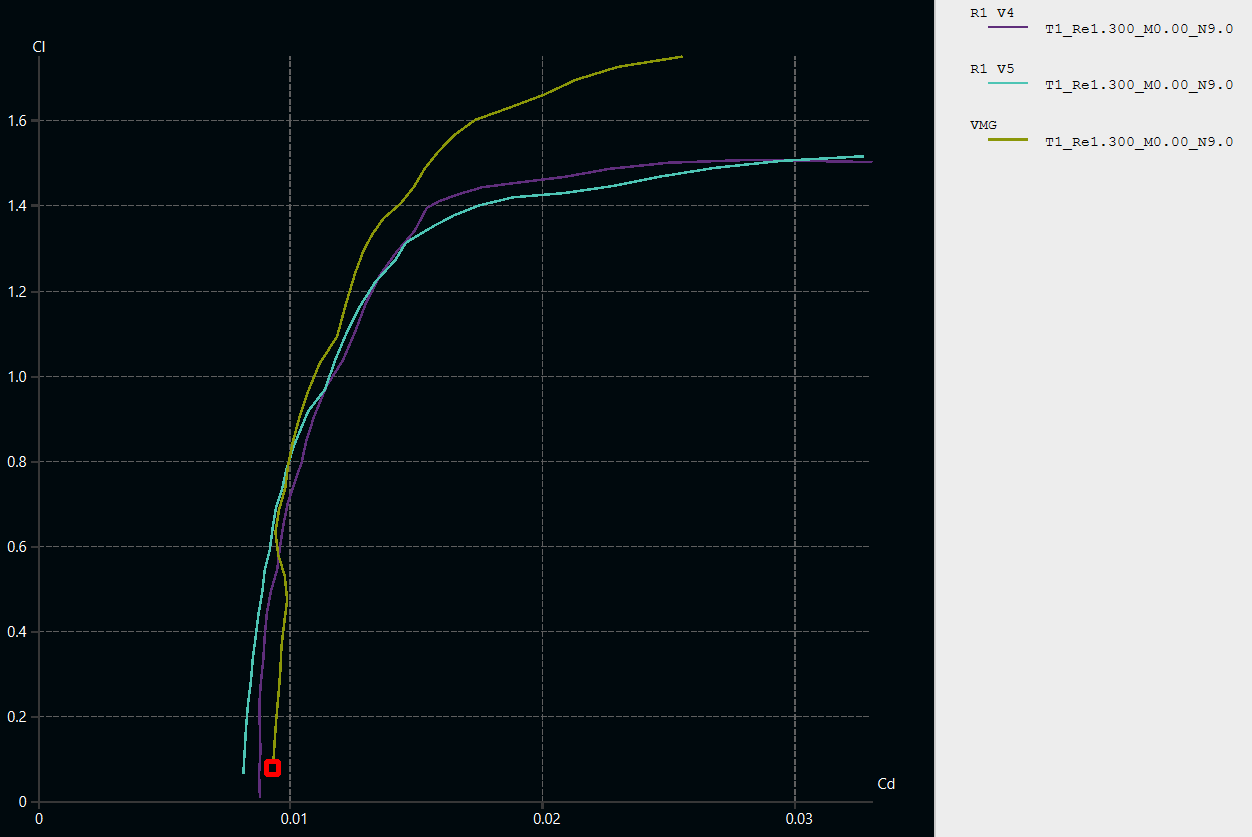
\includegraphics[width=0.5\textwidth]{figures/2D steady simulations/xflr5/Polar upwind.png}
    \caption{Upwind polars}
    \label{fig:Upwind_polars}
\end{figure}

Moreover, according to the team rider Axel Mazzela, "the R1 V4 is the one that does not fly enough to the edge of the wind window when the rider slacks (going upwind)". The lack of Cl (and therefore of finesse) in these conditions may be an explanation to that phenomena. 

However, these results need to be nuanced by the fact that at this stage the 3d effects are not taken into account.

For all the airfoils, the boundary layer transition from laminar to turbulent appears around 20$\%$ of the chord on the upper surface and 70$\%$ on the lower surface at an angle of attack of 5°. However, this result should be nuanced by the presence of seams along the leading edge of the kite, likely causing an earlier transition. Later in the internship, the transition had been deliberately induced to occur at the leading edge, and the comparison between the kites remained consistent.

%%
\vspace{1cm}
Then, the downwind polars have been plotted using a speed of 20 knots and a Reynolds number of $0,7e^{6}$

\begin{figure}[H]
\begin{subfigure}{0.5\textwidth}
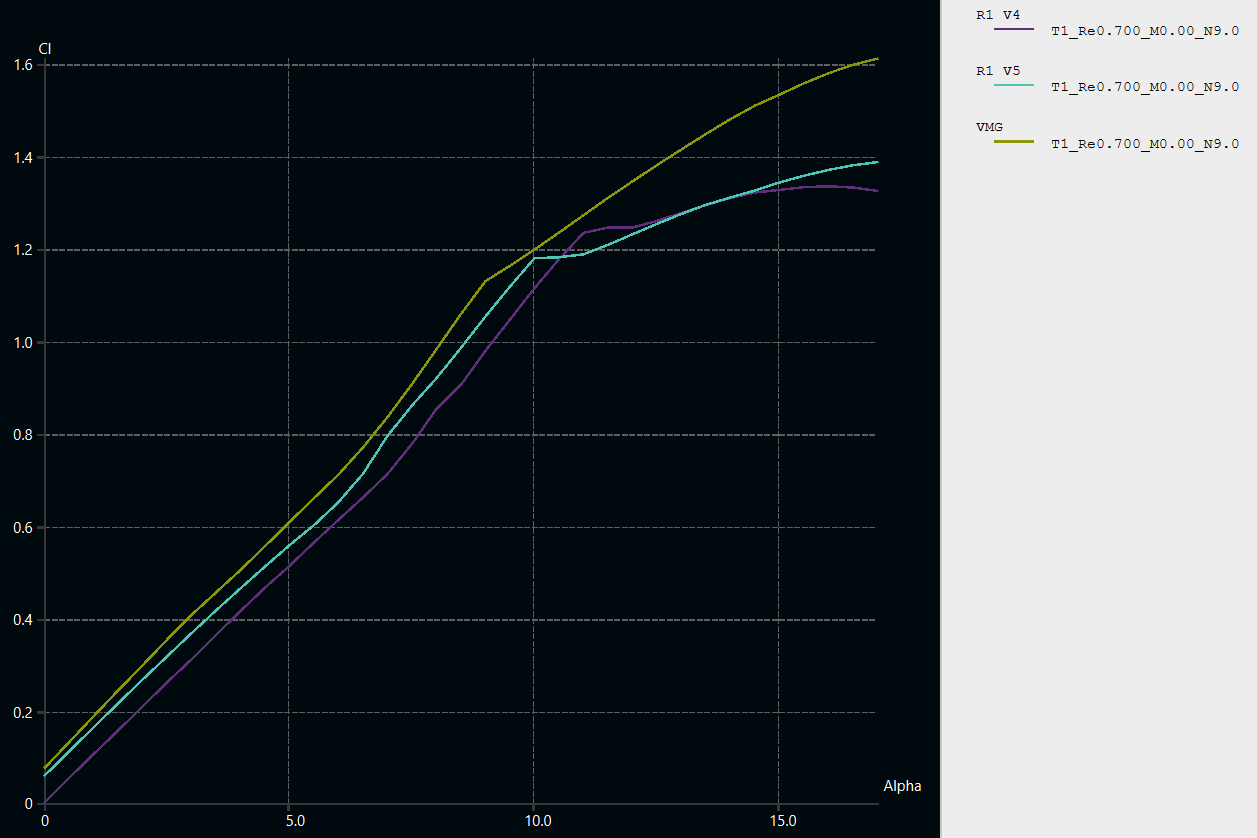
\includegraphics[width=1.\textwidth]{figures/2D steady simulations/xflr5/Cl downwind.png}
\caption{Plot of Cl downwind}
\label{fig:Plot_of_Cl_downwind}
\end{subfigure}
\begin{subfigure}{0.5\textwidth}
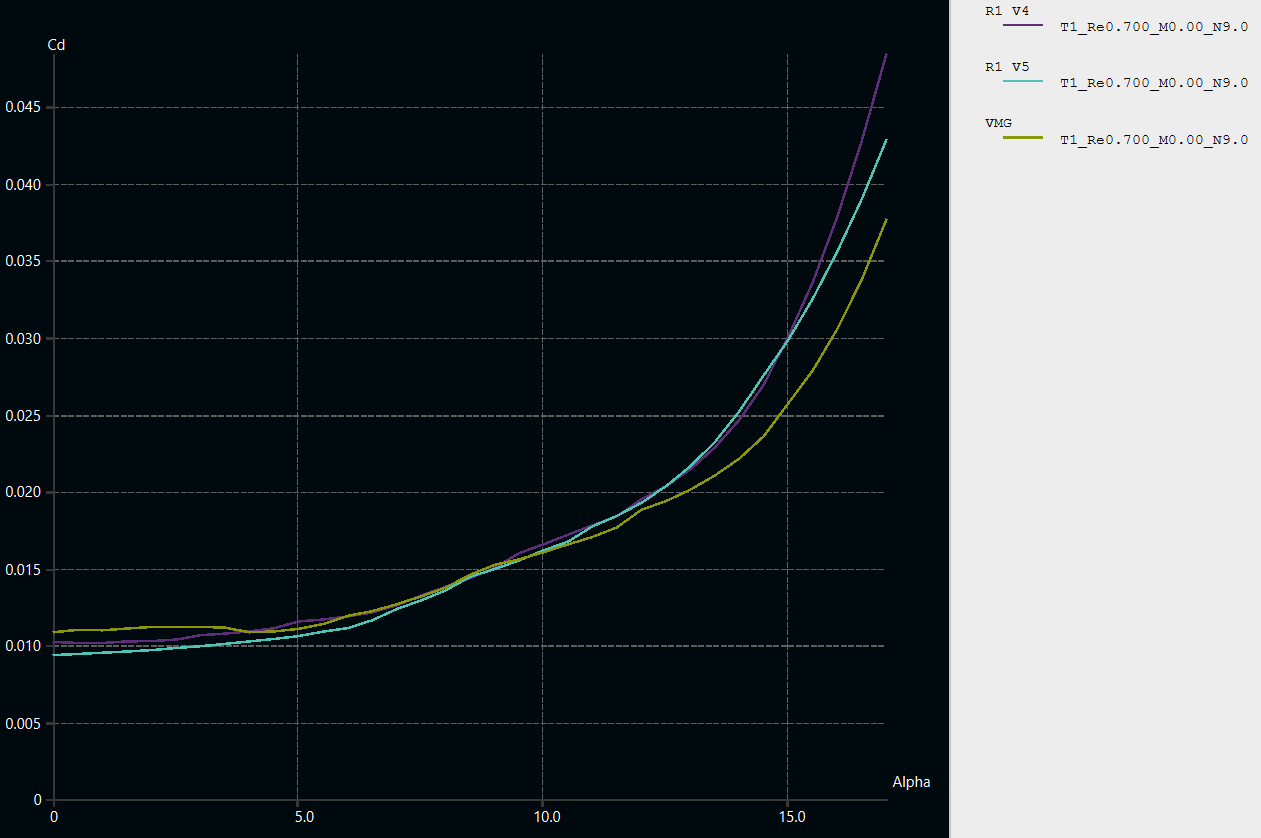
\includegraphics[width=1.\textwidth]{figures/2D steady simulations/xflr5/Cd Downwind.png}
\caption{Plot of Cd downwind}
\label{fig:Plot_of_Cd_downwind}
\end{subfigure}
\caption{Downwind plots}
\label{fig:Downwind_plots}
\end{figure}

These polars are interesting for higher angles of attack ( 7-14° according to \ref{tab:commonly_accepted_inlet_values} ) and need to be nuanced by the low reliability of XFLR5 at high angles of attack ( near the stall and post-stall ) \cite{XFOILlimits}. 


\begin{figure}[H]
    \centering
    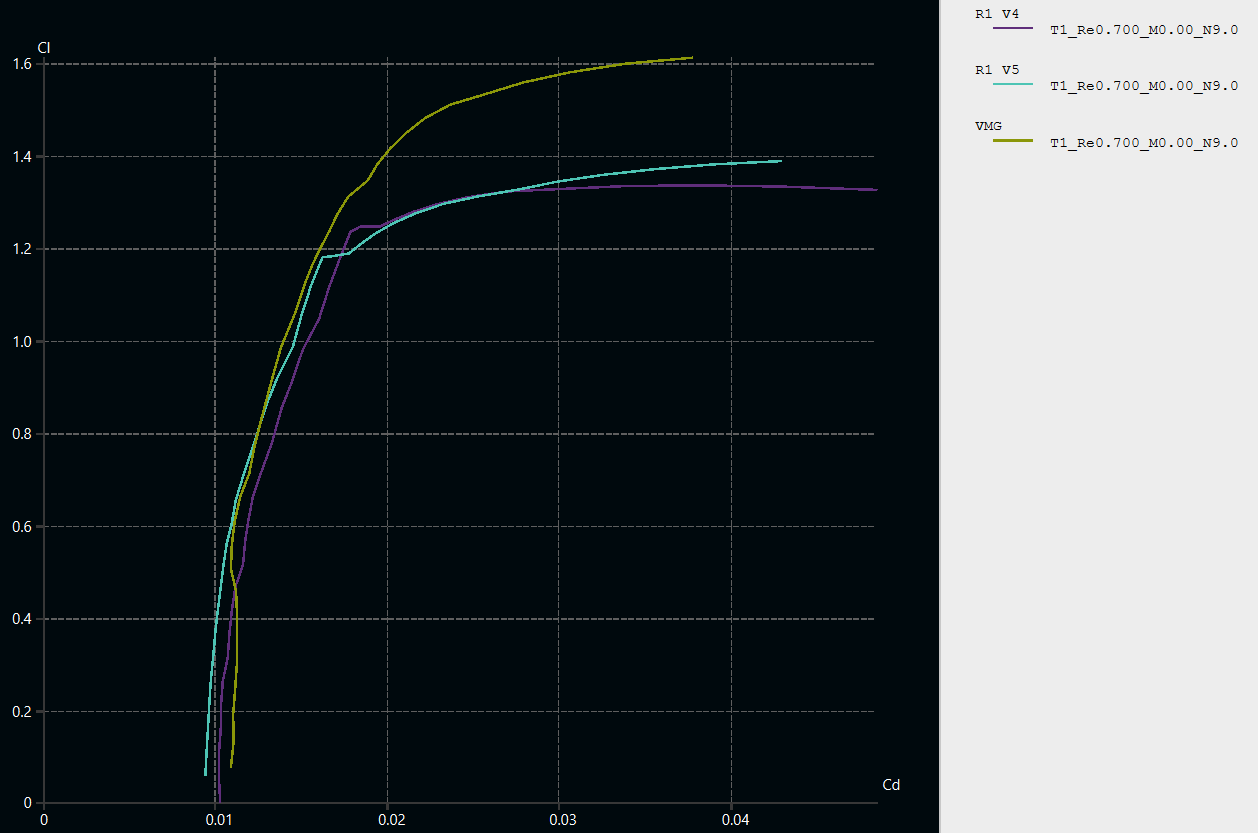
\includegraphics[width=0.5\textwidth]{figures/2D steady simulations/xflr5/Polar downwind.png}
    \caption{Downwind polars}
    \label{fig:Downwind_polars}
\end{figure}

We can see from these polars that the VMG has a higher Cl than the R1s and a lower Cd. 

According to Axel "the main issue with the R1 V5 is the low tether tension during this phase that can lead to a loose of tensions in the lines and its difficulty to fly forward when hauling the bar". 


Furthermore, comparing the R1 V4, which was only tested with three line sets, to the R1 V5 and the VMG, both of which were tested with only two line sets, proves challenging. In fact, Axel's observation suggests that with three lines, "the kite's shape is reinforced, and it catches the wind more quickly, resulting in a shorter transition time."

From this, it becomes apparent that the disparities in performance between the kites cannot be solely attributed to the airfoil design. Other factors, such as 3D effects and the number of lines, could provide a more comprehensive explanation for these results.

For all the airfoils, the boundary layer transition from laminar to turbulent appears around 16-19$\%$ of the chord on the upper surface and does not transit on the lower surface at an angle of attack of 10°. 

\textbf{From these results, and in connection with the experience of the team rider and both Ozone design teams (paraglider and kite), it appears that increasing the aerodynamic finesse of the R1 and enhancing lift in downwind conditions would enable them to surpass the VMG.}

%%%%%%%%%%%%%%%%%%%%%%%%%%%%%%%%%%%%%%%%%%%%%%%%%%%%%%%%%%%%%%%%%%%%%%%%%%%%%%%%
%%%%%%%%%%%%%%%%%%%%%%%%%%%%%%%%%%%% SECTION 5 %%%%%%%%%%%%%%%%%%%%%%%%%%%%%%%%%
%%%%%%%%%%%%%%%%%%%%%%%%%%%%%%%%%%%%%%%%%%%%%%%%%%%%%%%%%%%%%%%%%%%%%%%%%%%%%%%%

\section{The airfoil design}
\label{sec:Ch1.5}

Based on the preceding findings and in consultation with the Ozone design team, we generated the following Cp plot and conducted a comparative analysis of the foil designs in order to formulate our approach for the next airfoil prototype to be tested.

\begin{figure}[H]
\begin{subfigure}{0.5\textwidth}
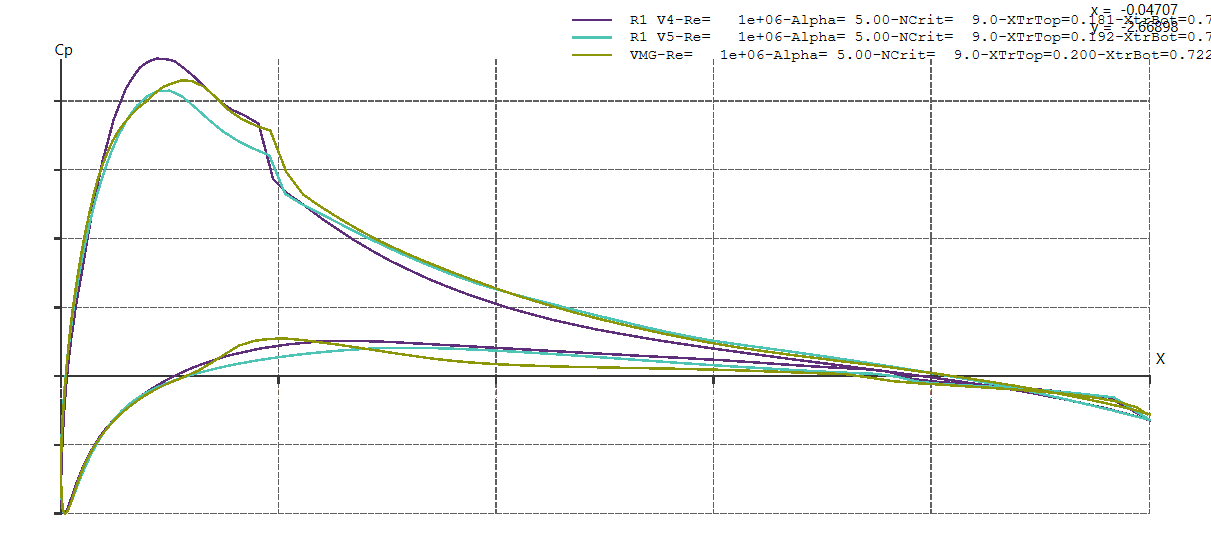
\includegraphics[width=1\textwidth]{figures/2D steady simulations/airfoil design/cp upwind 5deg.png}
\caption{Plot of Cp upwind at 5°}
\label{fig:Plot_of_Cp_upwind}
\end{subfigure}
\begin{subfigure}{0.5\textwidth}
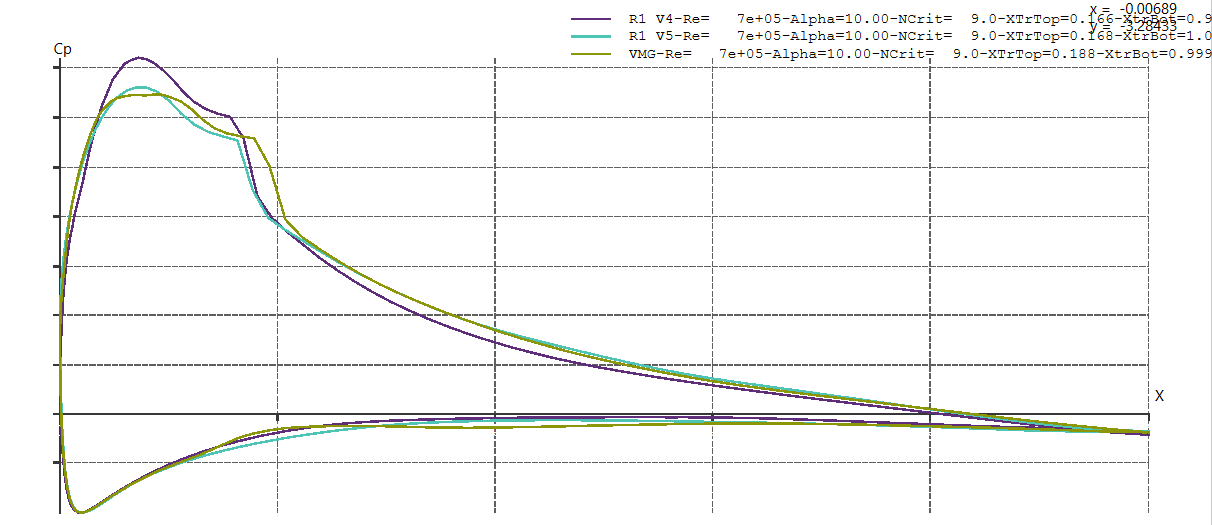
\includegraphics[width=1\textwidth]{figures/2D steady simulations/airfoil design/cp downwind 10deg.png}
\caption{Plot of Cp downwind at 10°}
\label{fig:Plot_of_Cp_downwind}
\end{subfigure}
\caption{Cp plots}
\label{fig:Cp_plots}
\end{figure}

We can see in the Cp plots that all kites have a peak of Cp on the upper surface near 10$\%$ of the chord then a boundary layer transition near 20$\%$ of the chord. However, if the R1 V4 has the highest peak, it also have a higher Cp on the lower surface which leads to a lower C$_{L}$. The R1 V5 has a lower Cp peak on the upper surface than the R1 V4 but also a lower Cp on the lower surface.

The VMG upper surface seems to be a good compromise between the three different Cp plot as its peak is lower than the R1 V4 but its turbulent part is higher.

However, the R1s' lower surfaces seem to be better than the VMG because they lead to mostly lower and smoother Cp plot.

\vspace{1cm}

If we consider the airfoils, we can see that the VMG lower surface reaches its lowest point earlier than the other airfoils which may lead too a smoother interaction between the intrados and extrados flows at the trailing edge (because its recompression zone is larger).

\begin{figure}[H]
    \centering
    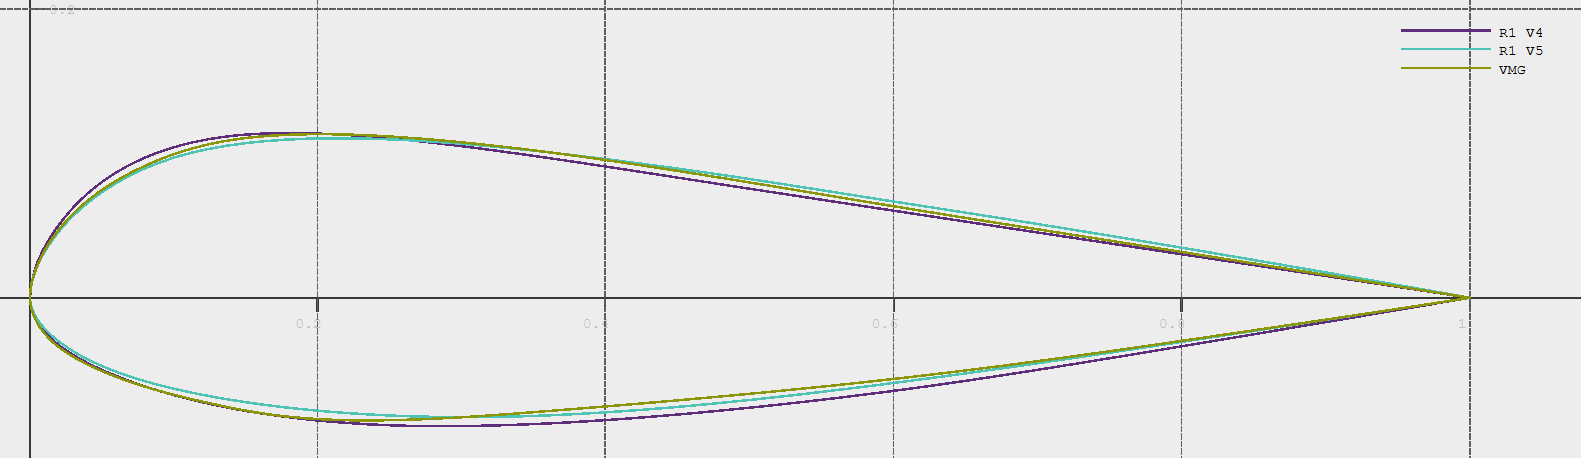
\includegraphics[width=0.8\textwidth]{figures/2D steady simulations/airfoil design/foils design.png}
    \caption{The 3 different airfoil designs}
    \label{fig:The_3_different_airfoil_designs}
\end{figure}

As a result, with the help of Rob Whittall, product designer, co-owner and co-founder of Ozone, we designed a new airfoil making the lower surface of the R1 V5 "smoother" and changing the VMG upper surface making its leading edge "rounder". The resulting airfoil was named "R1 V5 Satori 3". 

\begin{figure}[H]
\begin{subfigure}{1\linewidth}
\centering
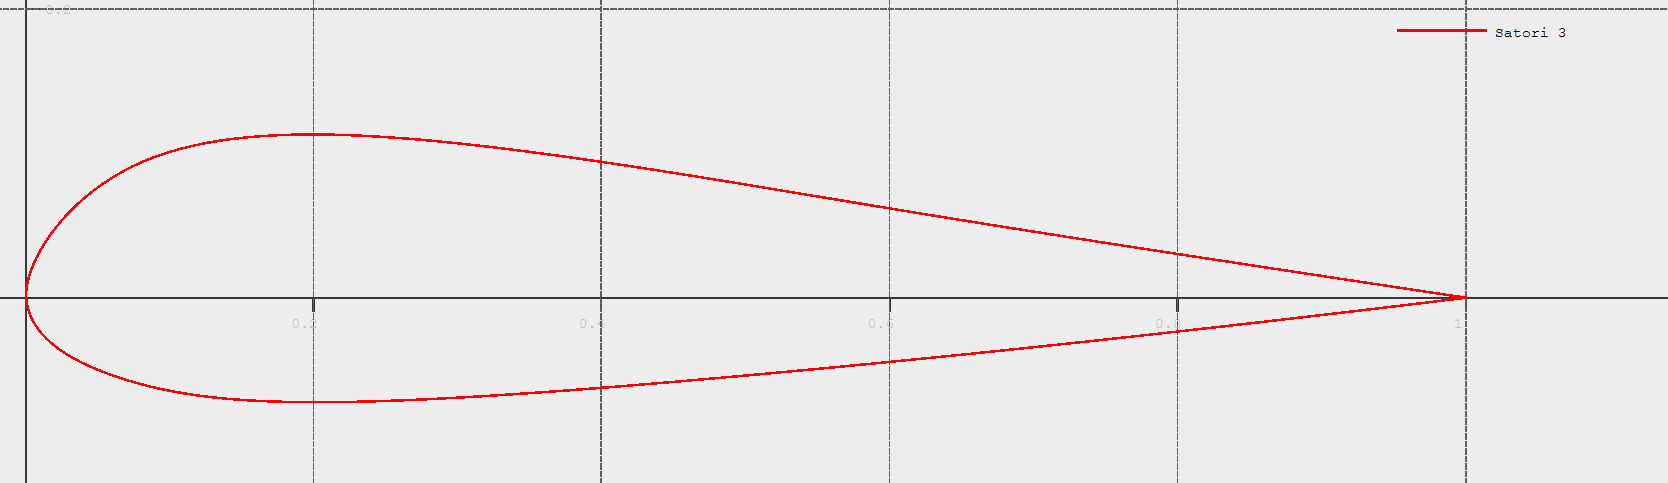
\includegraphics[width=0.9\textwidth]{figures/2D steady simulations/airfoil design/satori 3.png}
\caption{The R1 V5 Satori 3 airfoil}
\label{fig:The_R1_V5_Satori_3_airfoil}
\end{subfigure}
\centering
\begin{subfigure}{0.9\linewidth}
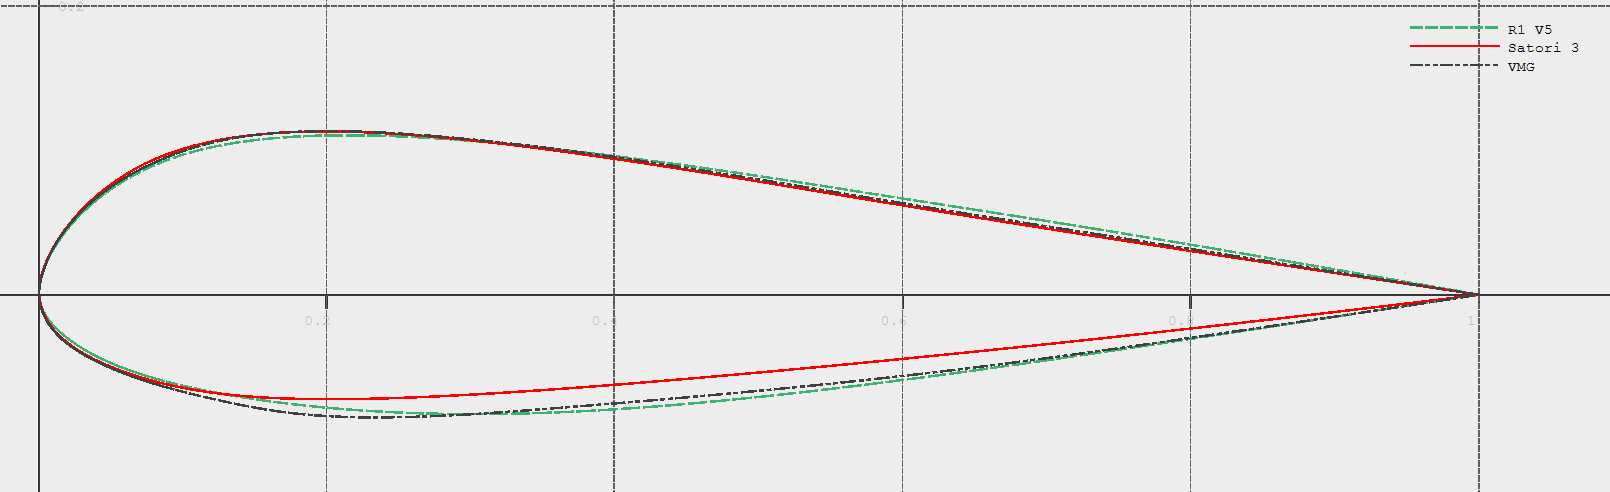
\includegraphics[width=1.\textwidth]{figures/2D steady simulations/airfoil design/satori 3, R1V5 and VMG.png}
\caption{The R1 V5 Satori 3, R1 V5 and VMG airfoils}
\label{fig:The_R1_V5_Satori_3,_R1_V5_and_VMG_airfoils}
\end{subfigure}
\caption{Cp plots}
\label{fig:Comparison between different airfoil designs}
\end{figure}

The following graphs \ref{fig:Cd_Cl_plot_of_the_VMG_and_R1_V5_Satori_3} and \ref{fig:Polar_of_the_VMG_and_R1_V5_Satori_3} show that the R1 V5 Satori 3 has a higher Cl, lower Cd and, as a result, a higher finesse upwind at 5° and downwind at 10°. 

\begin{figure}[H]
\begin{subfigure}{0.5\textwidth}
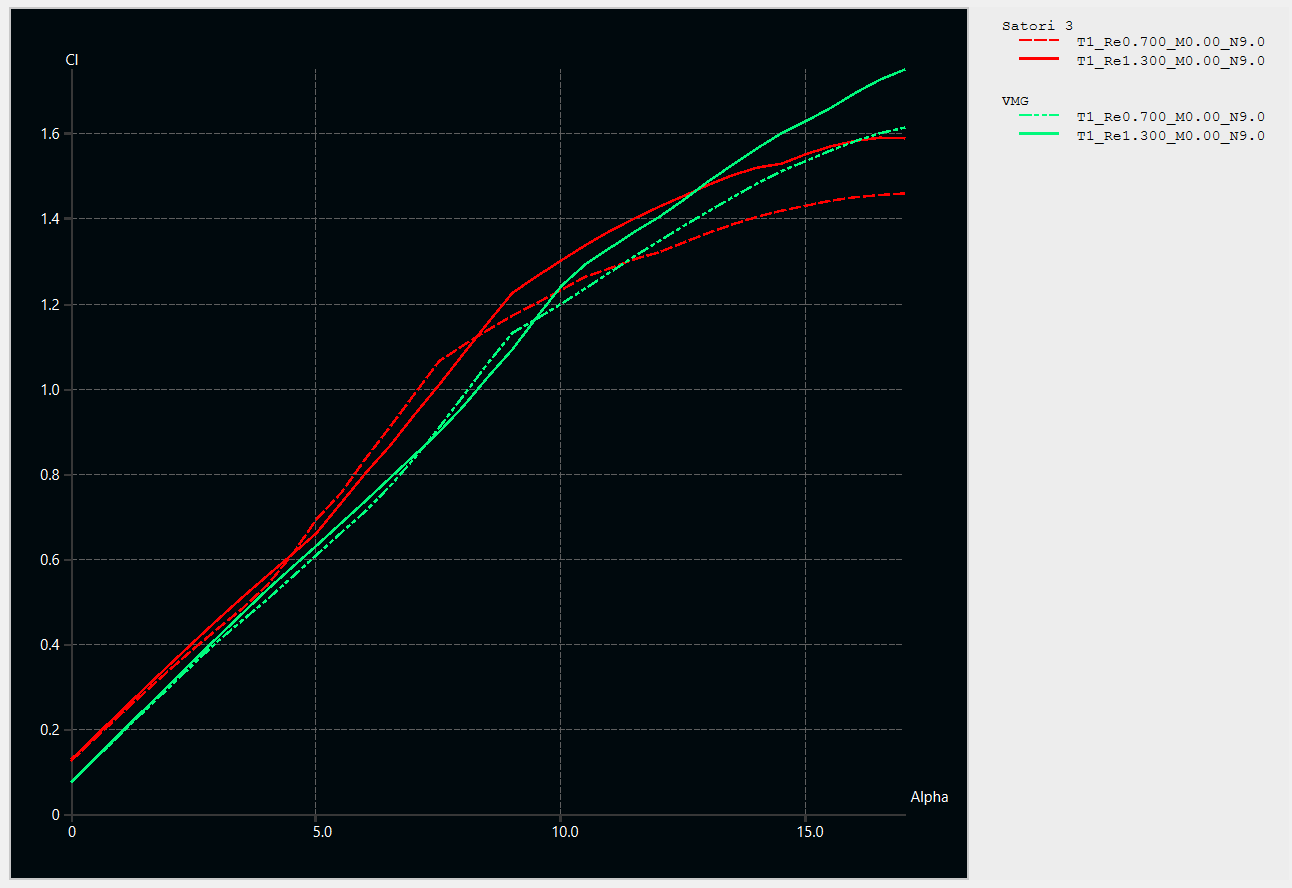
\includegraphics[width=1\textwidth]{figures/2D steady simulations/xflr5/Cl vmg sat3.png}
\caption{Cl plot}
\label{fig:Cl_plot_of_the_VMG_and_R1_V5_Satori_3}
\end{subfigure}
\begin{subfigure}{0.5\textwidth}
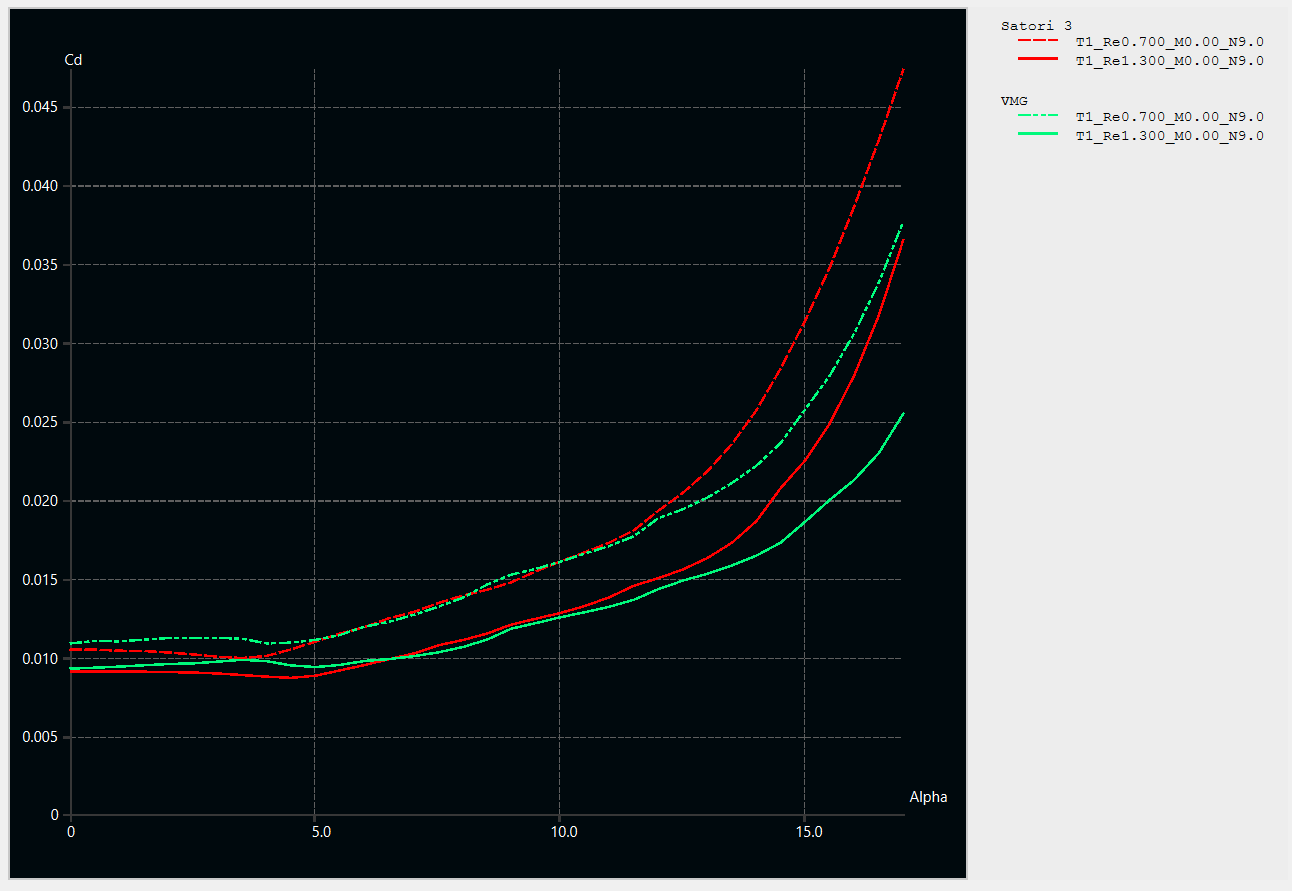
\includegraphics[width=1\textwidth]{figures/2D steady simulations/xflr5/Cd vmg sat3.png}
\caption{Cd}
\label{fig:Cd_plot_of_the_VMG_and_R1_V5_Satori_3}
\end{subfigure}
\caption{Cd $\&$ Cl plots (VMG and R1 V5 Satori 3)}
\label{fig:Cd_Cl_plot_of_the_VMG_and_R1_V5_Satori_3}
\end{figure}

\begin{figure}[H]
    \centering
    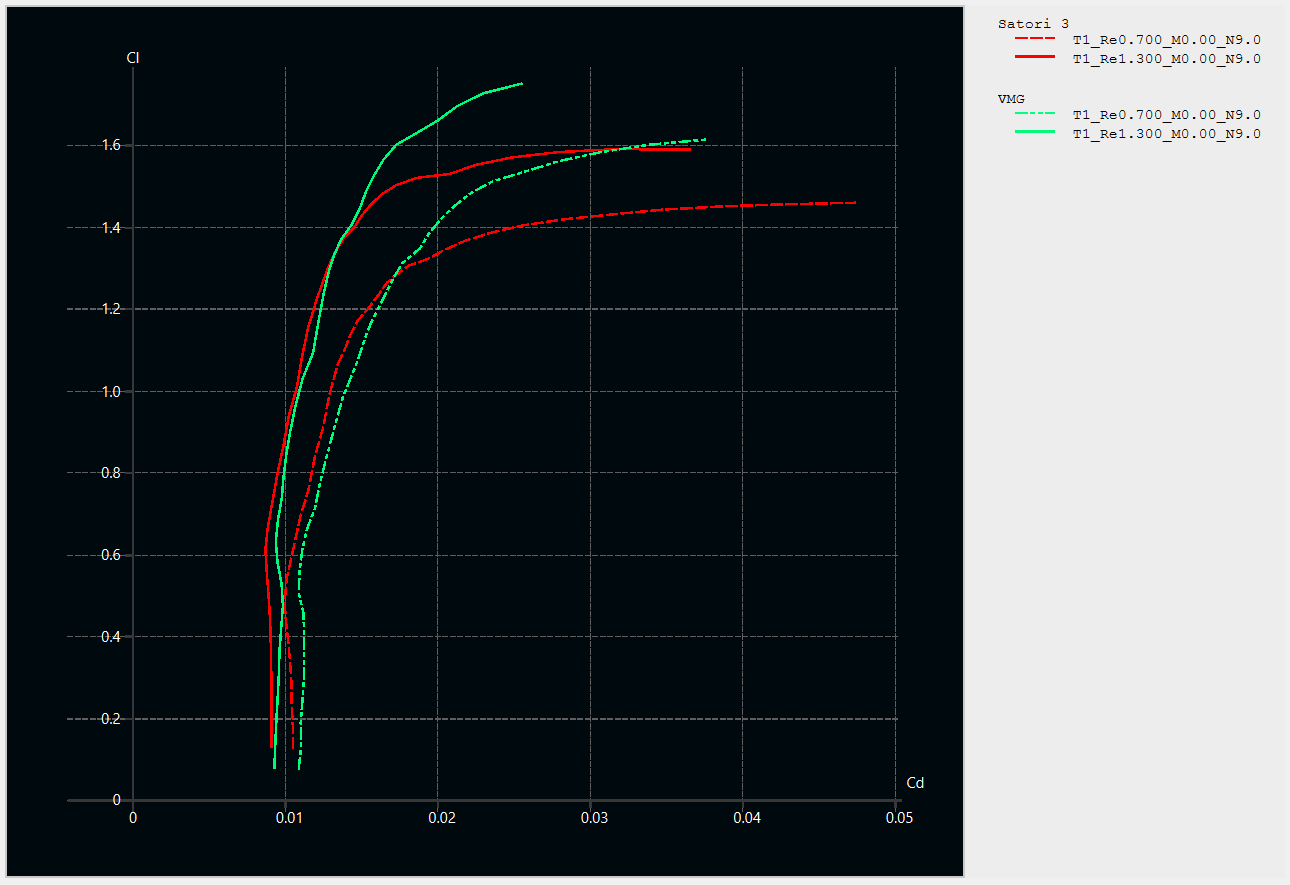
\includegraphics[width=0.75\textwidth]{figures/2D steady simulations/xflr5/polar vmg sato3.png}
    \caption{Polars (VMG and R1 V5 Satori 3)}
    \label{fig:Polar_of_the_VMG_and_R1_V5_Satori_3}
\end{figure}

Moreover, we can see on the figure \ref{fig:Cp_plots_of_VMG_and_R1_V5_Satori_3} that the objectives in term of Cp plot have been reached. 

\begin{figure}[H]
    \begin{subfigure}{0.5\linewidth}
    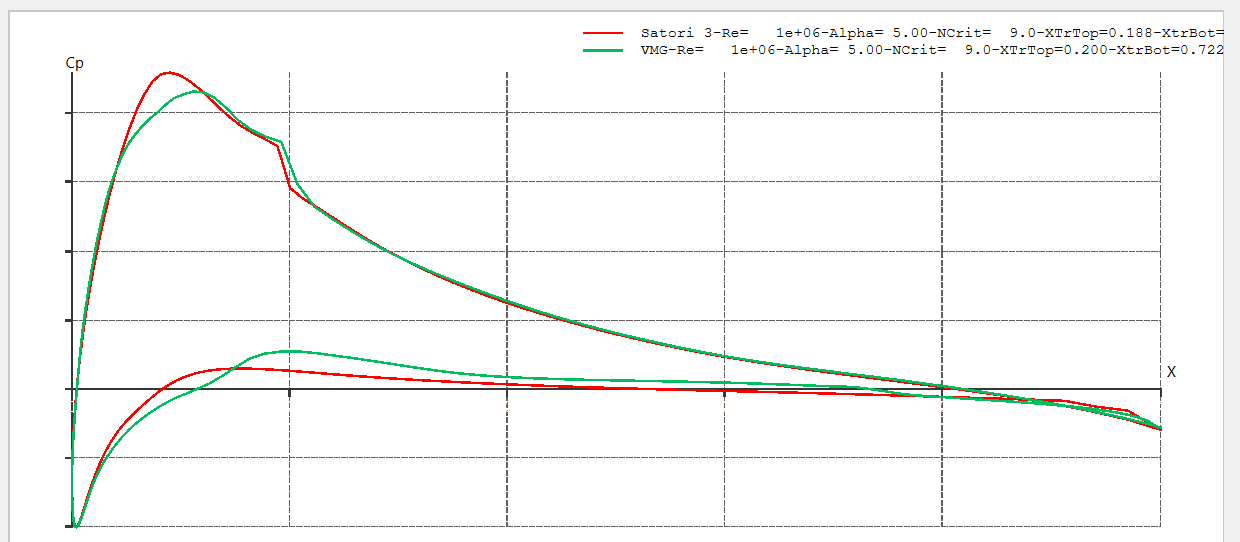
\includegraphics[width=1.\linewidth]{figures/2D steady simulations/airfoil design/cp upwind 5deg vmg sato3.png}
    \caption{Cp plot upwind at 5°}
    \label{fig:Cp_plot_upwind_at_5°}
    \end{subfigure}
    \begin{subfigure}{0.5\linewidth}
    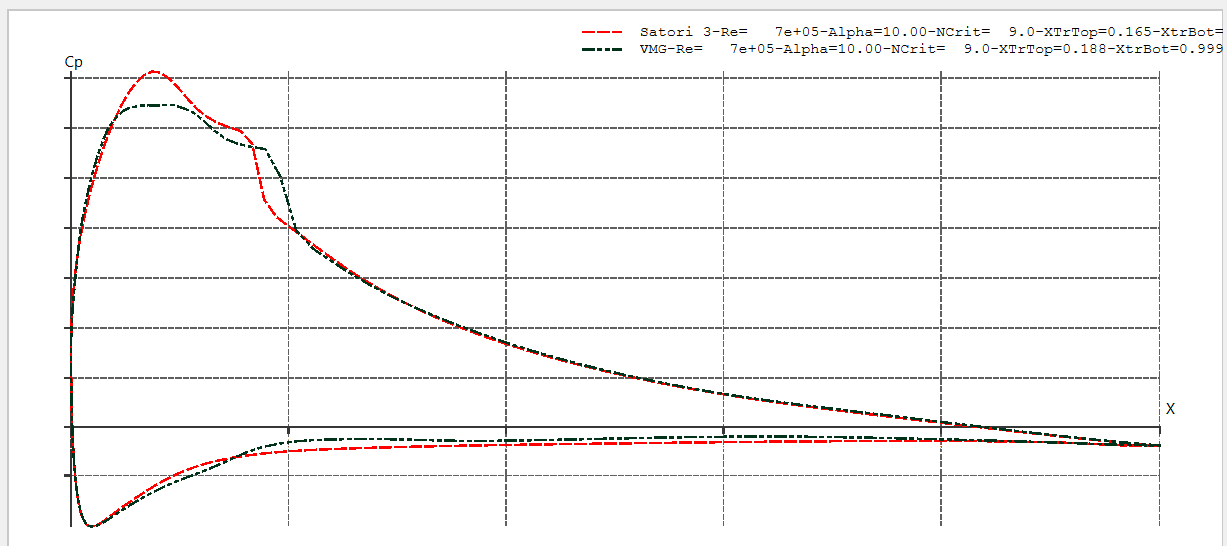
\includegraphics[width=1.\linewidth]{figures/2D steady simulations/airfoil design/cp downwind 10deg vmg sato3.png}
    \caption{Cp plot downwind at 10°}
    \label{fig:Cp_plot_downwind_at_10°}
    \end{subfigure}
    \caption{Cp plots of VMG and R1 V5 Satori 3}
\label{fig:Cp_plots_of_VMG_and_R1_V5_Satori_3}
\end{figure}

%%%%%%%%%%%%%%%%%%%%%%%%%%%%%%%%%%%%%%%%%%%%%%%%%%%%%%%%%%%%%%%%%%%%%%%%%%%%%%%%
%%%%%%%%%%%%%%%%%%%%%%%%%%%%%%%%%%%% SECTION 6 %%%%%%%%%%%%%%%%%%%%%%%%%%%%%%%%%
%%%%%%%%%%%%%%%%%%%%%%%%%%%%%%%%%%%%%%%%%%%%%%%%%%%%%%%%%%%%%%%%%%%%%%%%%%%%%%%%

\section{FLUENT - The 2D steady simulations}
\label{sec:Ch1.6}

%%%%%%%%%%%%%%%%%%%%%%%%%%%%%%%%%%%% SUBSECTION 1

\subsection{The spatial convergence}
\label{sub:Ch1.6.1}

We conducted comparisons using ANSYS FLUENT to refine the results. The objective was to provide Ozone with a more precise comprehension of the flow characteristics around their airfoils and accurate aerodynamic coefficients, particularly in the vicinity of the stall, where XFLR5 is recognized to be less reliable. 

The meshing was done using the FLUENT meshing software. For a flow speed from 20 to 35 knots and $y{+} = 1$, $\delta y = 3.4e^{-5}$ to $2e^{-5}$. These value were respected.

Furthermore, spatial merging has been confirmed for all airfoil designs. To illustrate, consider the R1 V5 Satori 3, which yielded the following results: 

\begin{table}[H]
    \center
    \begin{tabular}{|l|l|l|l|}
        \hline
        number of elements & 138653 & 200150 & 288180 \tabularnewline
        \hline
        CL & 0,1276 & 0,1272 & 0,1258  \tabularnewline
        \hline
        CD & 0,0124 & 0,01245 & 0,0124  \tabularnewline
        \hline
        Finesse & 10,2903 & 10,2169 & 10,1452  \tabularnewline
        \hline
    \end{tabular}
    \caption{R1 V5 Satori 3 results at O° and 30 knots}
    \label{tab:R1_V5_results_at_O°_and_35_knots}
\end{table}

Then, using the Richardson interpolation method \cite{RichardsonInterpolation}:

\begin{equation}
\left \{
   \begin{array}{r c l}
      p  & = & \frac{1}{ln(r)} \frac{ln(m_{3}-m_{2})}{ln(m_{2}-m_{1})} \\
      m^{*}   & = & \frac{m_{3}-m_{2}r^{p}}{1-r^{p}} \\
   \end{array}
   \right .
   \label{Richardson_interpolation}
\end{equation}
(with $m_{i}$ the results obtained for meshes with element sizes in a ratio r, $m^{*}$ the asymptotic value and p the merging order)

We obtain : 

\begin{table}[H]
    \center
    \begin{tabular}{|l|l|l|l|}
        \hline
           & p & Asymptotic value & Required accuracy \tabularnewline
        \hline
        CL & 2,30 &  0,1247 & $e^{-2}$ \tabularnewline
        \hline
        CD & 2,73 & 0,0124 & $e^{-3}$ \tabularnewline
        \hline
        Finesse & 2,76 & 10,1452 &  $e^{0}$ \tabularnewline
        \hline
    \end{tabular}
    \caption{R1 V5 asymptotic results at O° and 30 knots}
    \label{tab:R1_V5_asymptotic_results_at_O°_and_35_knots}
\end{table}

\begin{figure}[H]
    \centering
    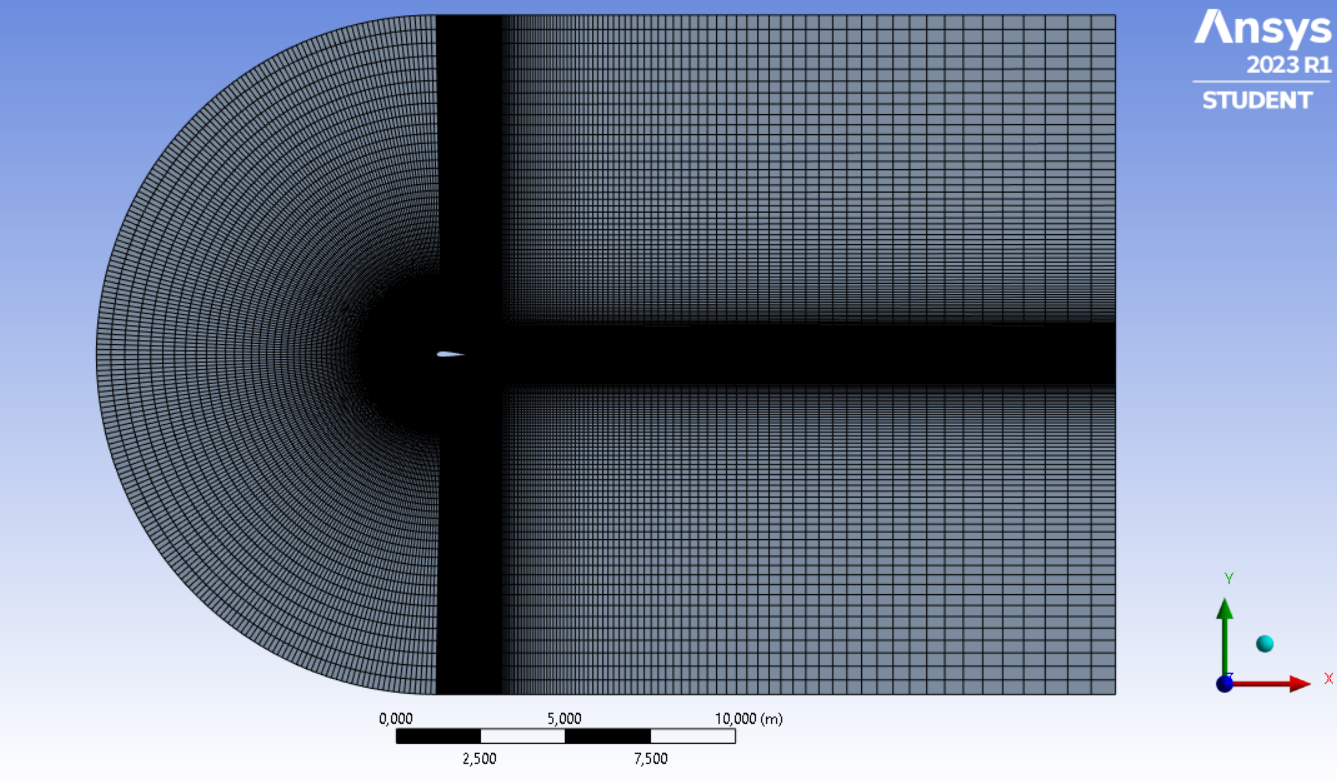
\includegraphics[width=1\textwidth]{figures/2D steady simulations/fluent/R1 V5 meshing.png}
    \caption{The global meshing under FLUENT}
    \label{fig:The global meshing}
\end{figure}

\begin{figure}[H]
    \centering
    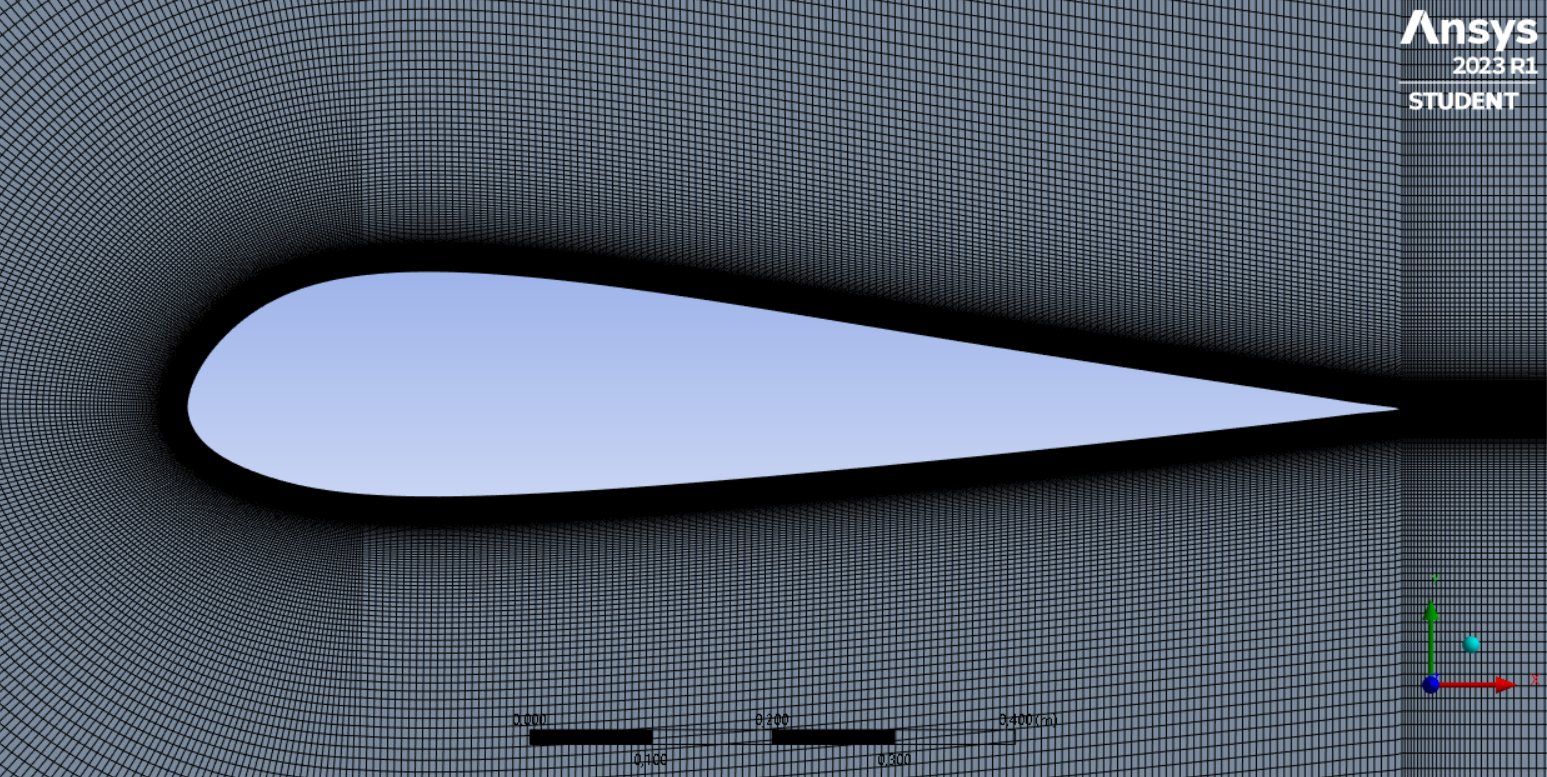
\includegraphics[width=0.75\textwidth]{figures/2D steady simulations/fluent/R1 V5 meshing zoom.png}
    \caption{Zoom on the airfoil}
    \label{fig:Zoom on the meshing}
\end{figure}


%%%%%%%%%%%%%%%%%%%%%%%%%%%%%%%%%%%% SUBSECTION 2

\subsection{The turbulence models}
\label{sub:Ch1.6.2}

FLUENT offers various turbulence models. 

Two models were tested to nuance the results :
\begin{itemize}
    \item \textbf{Spalart-Allmaras : } \\
    it is the only example of a transport equation model for $\nu_{t}$ used in the industry. This model is widely used in aeronautics for various reasons: It is easy to numerically integrate, for attached flows, it produces results as good as zero-equation models, and for separated flows, it provides a much better description of the velocity field than zero-equation models. However, this model is too simple (a single equation) to be valid for a wide range of flows \cite{turbulentmodels}.
    \item \textbf{k-$\omega$ SST : } \\
    The idea is to formulate a set of equations that converge towards the k-$\omega$ model near the wall and towards the k-$\epsilon$ model far from the walls. This model has been successfully applied in many configurations. It is currently one of the preferred models in the aerospace industry.
    k-$\omega$ provides better results than the standard k-$\epsilon$ and model in adverse pressure gradient situations, allowing for a more accurate prediction of separation points. The k-$\epsilon$ and k-$\omega$ models use two scales, not just one, so the aim is to overcome the limitations of the Spalart-Allmaras model.
    However, this first-order linear model comes with several assumptions :
    \begin{itemize}
        \item instantaneity, where the deformation and turbulence history have no influence
        \item locality, where turbulence is influenced only by its immediate surroundings.
        \item materially simple environment
        \item linearity of the behavior law
    \end{itemize}
    It is understood, then, that first-order linear models cannot work in all situations \cite{turbulentmodels}.
\end{itemize}

The figures \ref{fig:polars comparison between turbulence models on the R1 V5 Satori 3} and \ref{fig:Finesse relative error between turbulence models} compares the R1 V5 Satori 3 finesse plot at 35 knots with the two turbulence models. While the k-$\omega$ SST model is designed to provide more precise outcomes compared to the Spalart-Allmaras model, it introduces an elevated computational expense and an added difficulty in attaining spatial convergence. This is in contrast to the Spalart-Allmaras model, which generally converges toward a solution (that has spatially converged). Additionally, at low angles of attack, both models produce similar outcomes. It is only when encountering high angles of attack that noticeable disparities in results arise, reaching approximately 15\% divergence.

\begin{figure}[H]
    \centering
    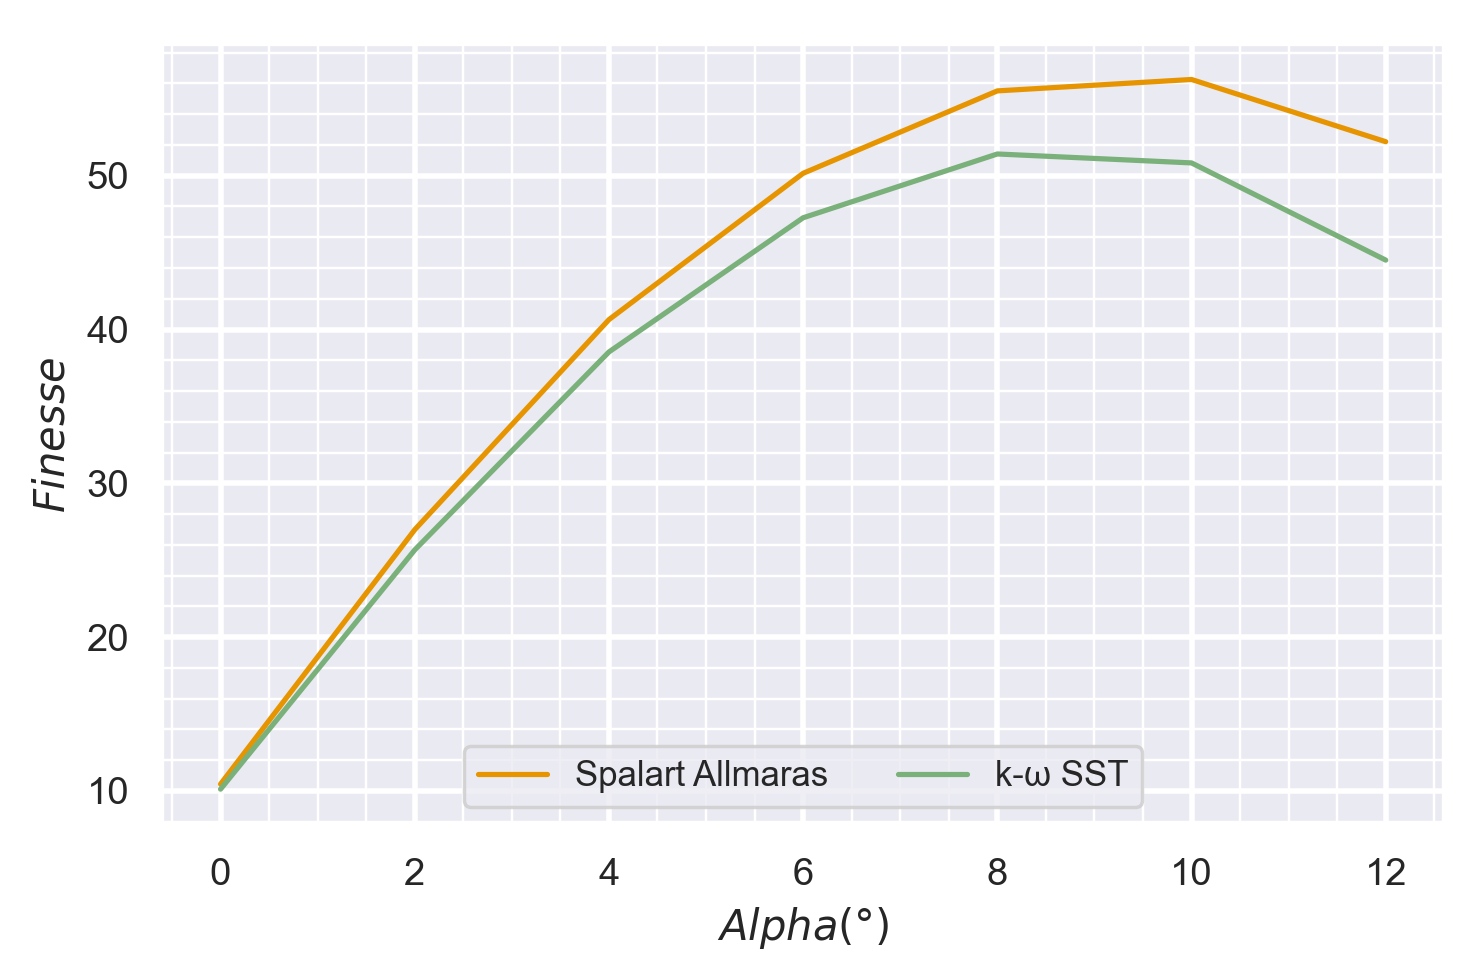
\includegraphics[width=0.75\linewidth]{figures/2D steady simulations/fluent/R1V5Satori3 Spalart Allmaras VS KWSST.png}
    \caption{finesse against alpha}
    \label{fig:polars comparison between turbulence models on the R1 V5 Satori 3}
\end{figure}

\begin{figure}[H]
    \centering
    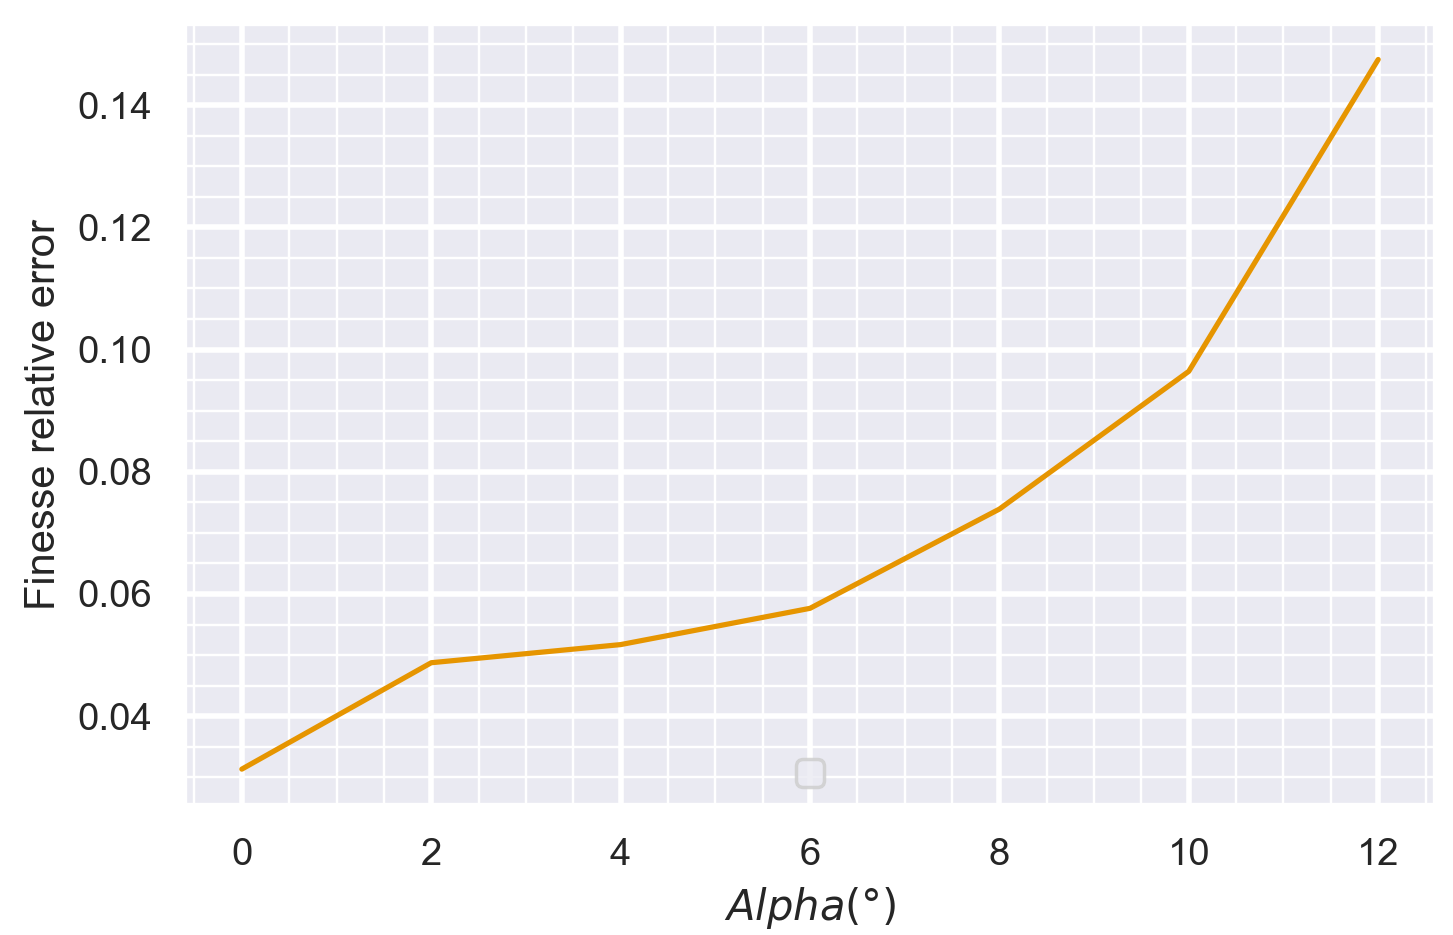
\includegraphics[width=0.75\linewidth]{figures/2D steady simulations/fluent/finesse relative error turbulence model.png}
    \caption{Finesse relative error against alpha}
    \label{fig:Finesse relative error between turbulence models}
\end{figure}

As a result, knowing the level of accuracy Ozone was looking for and the computational cost we could afford, \textbf{the Spalart-Allmaras model is the one we chose for our simulations}. 

\textbf{It's important to note that Ozone Kitesurf didn't seek highly precise results. Their primary objective was to gain insights into enhancing their existing airfoil while obtaining results that align with overall trends. Additionally, due to the computational limitations of my computer and the recognized influences of 3D effects, unsteadiness and fluid structure interactions, the pursuit of more precise results became less appealing.}

%%%%%%%%%%%%%%%%%%%%%%%%%%%%%%%%%%%% SUBSECTION 3

\subsection{The results}
\label{sub:Ch1.6.3}

The following figure \ref{fig:The R1 V5 meshing under FLUENT} shows the finesse plots for the R1 V5, R1 V5 Satori 3 and the VMG at 15 knots, the downwind conditions, and 35 knots, the upwind conditions. 

\begin{figure}[H]
    \begin{subfigure}{0.5\textwidth}
    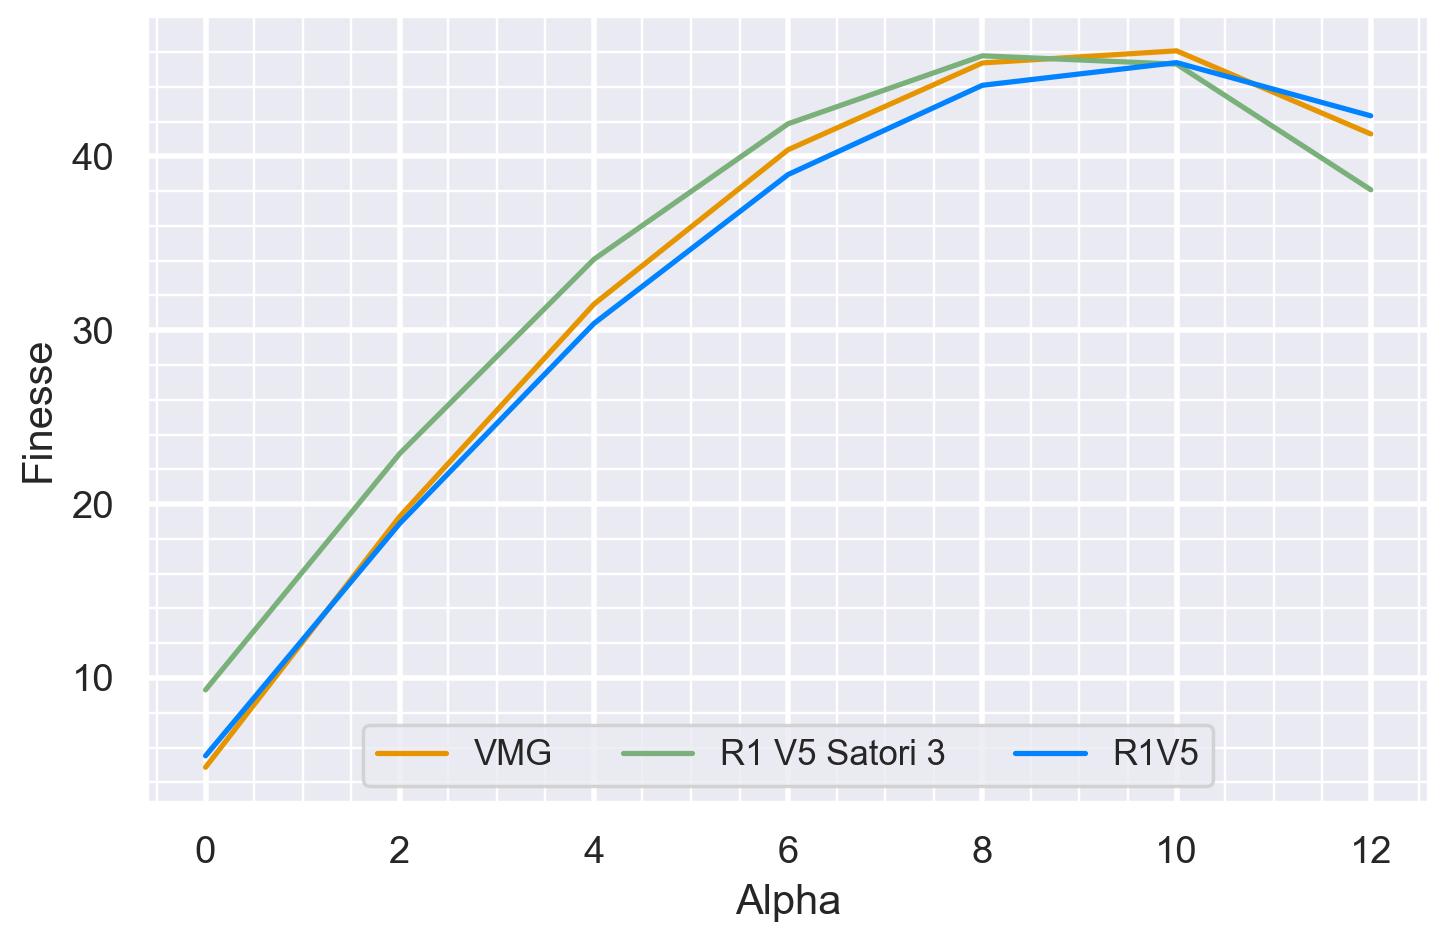
\includegraphics[width=1\textwidth]{figures/2D steady simulations/fluent/finesse VMG SAT3 R1V5 15kts FLUENT.png}
    \caption{15 knots}
    \label{fig:15 knots}
    \end{subfigure}
    \begin{subfigure}{0.5\textwidth}
    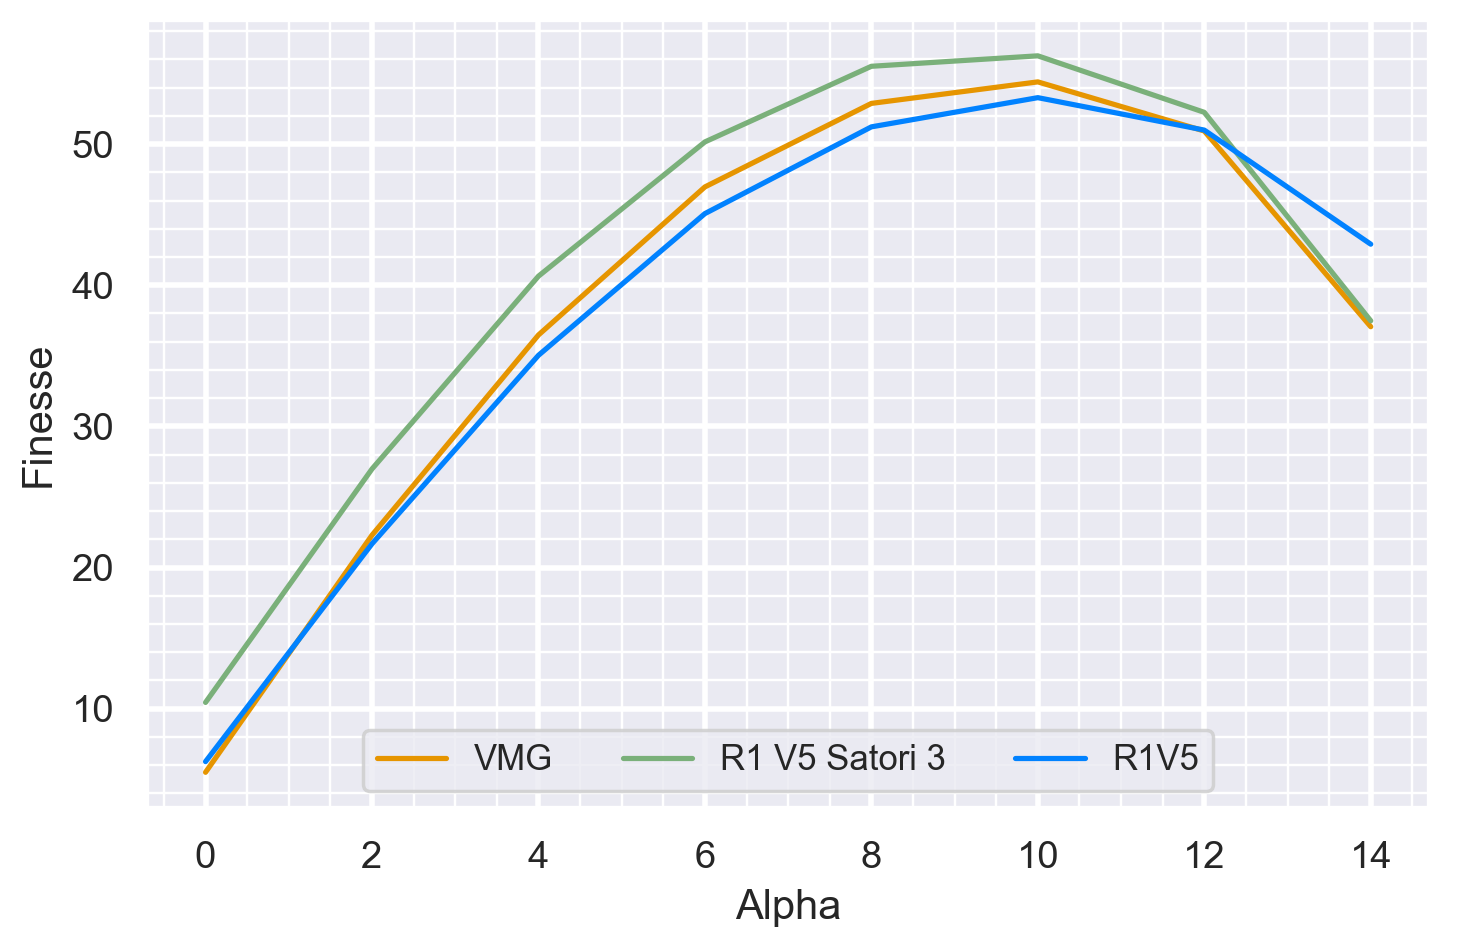
\includegraphics[width=1\textwidth]{figures/2D steady simulations/fluent/finesse VMG SAT3 R1V5 35kts FLUENT.png}
    \caption{35 knots}
    \label{fig:35 knots}
    \end{subfigure}
    \caption{R1 V5, R1 V5 Satori 3 \& VMG polars with FLUENT}
\label{fig:The R1 V5 meshing under FLUENT}
\end{figure}

These findings are rather promising, as we anticipate that the R1 V5 Satori3 will demonstrate enhanced performance in upwind conditions, particularly at low angles of attack, at 35 knots. Furthermore, in downwind scenarios, the R1 V5 Satori3 is projected to deliver favorable outcomes within the range of 5° to 8° angles of attack, but it is expected to experience a stall around 9-10°..  

\begin{figure}[H]
    \begin{subfigure}{0.5\textwidth}
    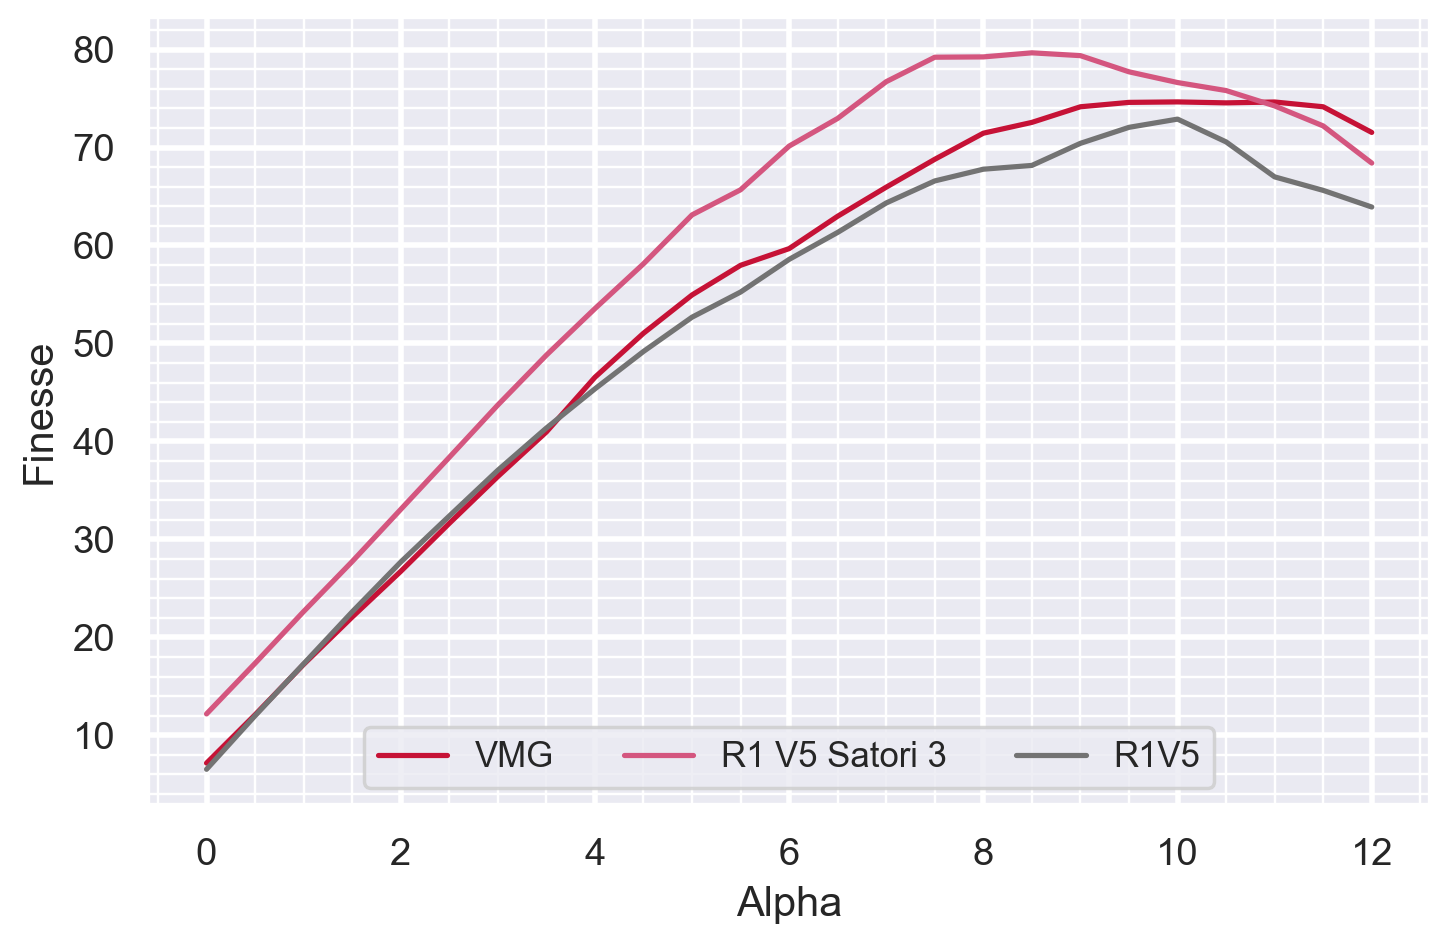
\includegraphics[width=1\textwidth]{figures/2D steady simulations/fluent/finesse VMG SAT3 R1V5 15kts XFLR5.png}
    \caption{15 knots}
    \label{fig:15 knots XFLR5}
    \end{subfigure}
    \begin{subfigure}{0.5\textwidth}
    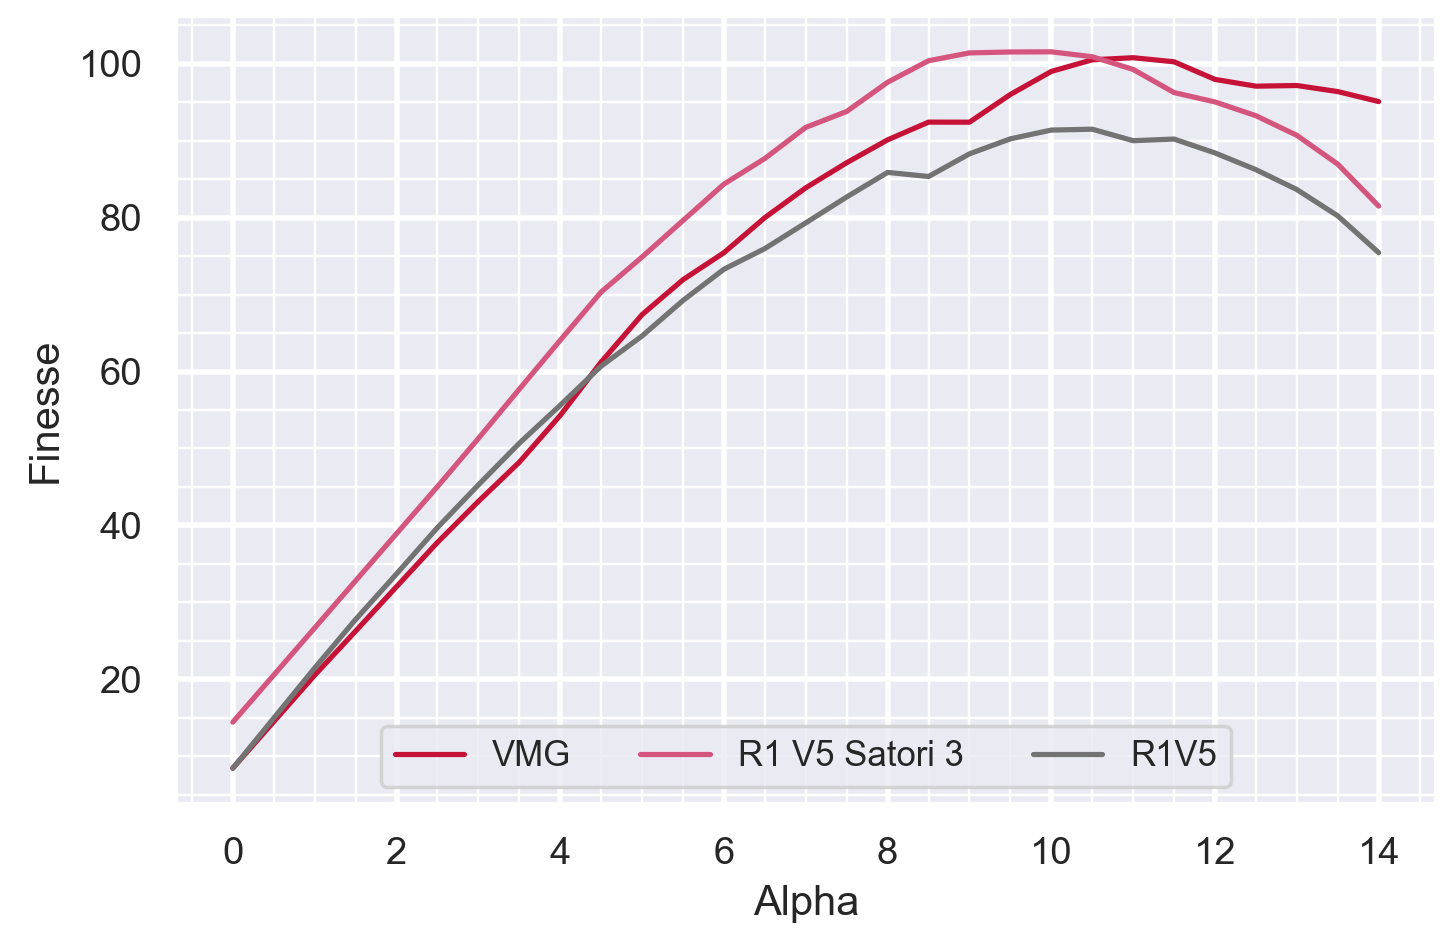
\includegraphics[width=1\textwidth]{figures/2D steady simulations/fluent/finesse VMG SAT3 R1V5 35kts XFLR5.png}
    \caption{35 knots}
    \label{fig:35 knots XFLR5}
    \end{subfigure}
    \caption{R1 V5, R1 V5 Satori 3 \& VMG polars with XFLR5}
\label{fig:The R1 V5 meshing under XFLR5}
\end{figure}

We also recognize the necessity of utilizing Fluent for simulations to achieve greater result accuracy, particularly when approaching the stall at high angles of attack. In fact, XFLR5 tends to provide higher estimates for the finesse values but is valuable for quickly obtaining initial insights into the relative behaviors of airfoils.

\textbf{The precision and cost-effectiveness of XFLR5 prompted, after extensive discussions with the paraglider design team, the initiation of a project to apply XFLR5's theories to simulate 3D effects and implement an optimization algorithm. This project is the central focus of Chapter \ref{Chapter2}.}

Consequently, we opted to initiate the development of a prototype for the R1 V5 Satori 3 and dispatch the kite to France for testing by the team riders to obtain their feedback on its performance.

\begin{figure}[H]
    \centering
    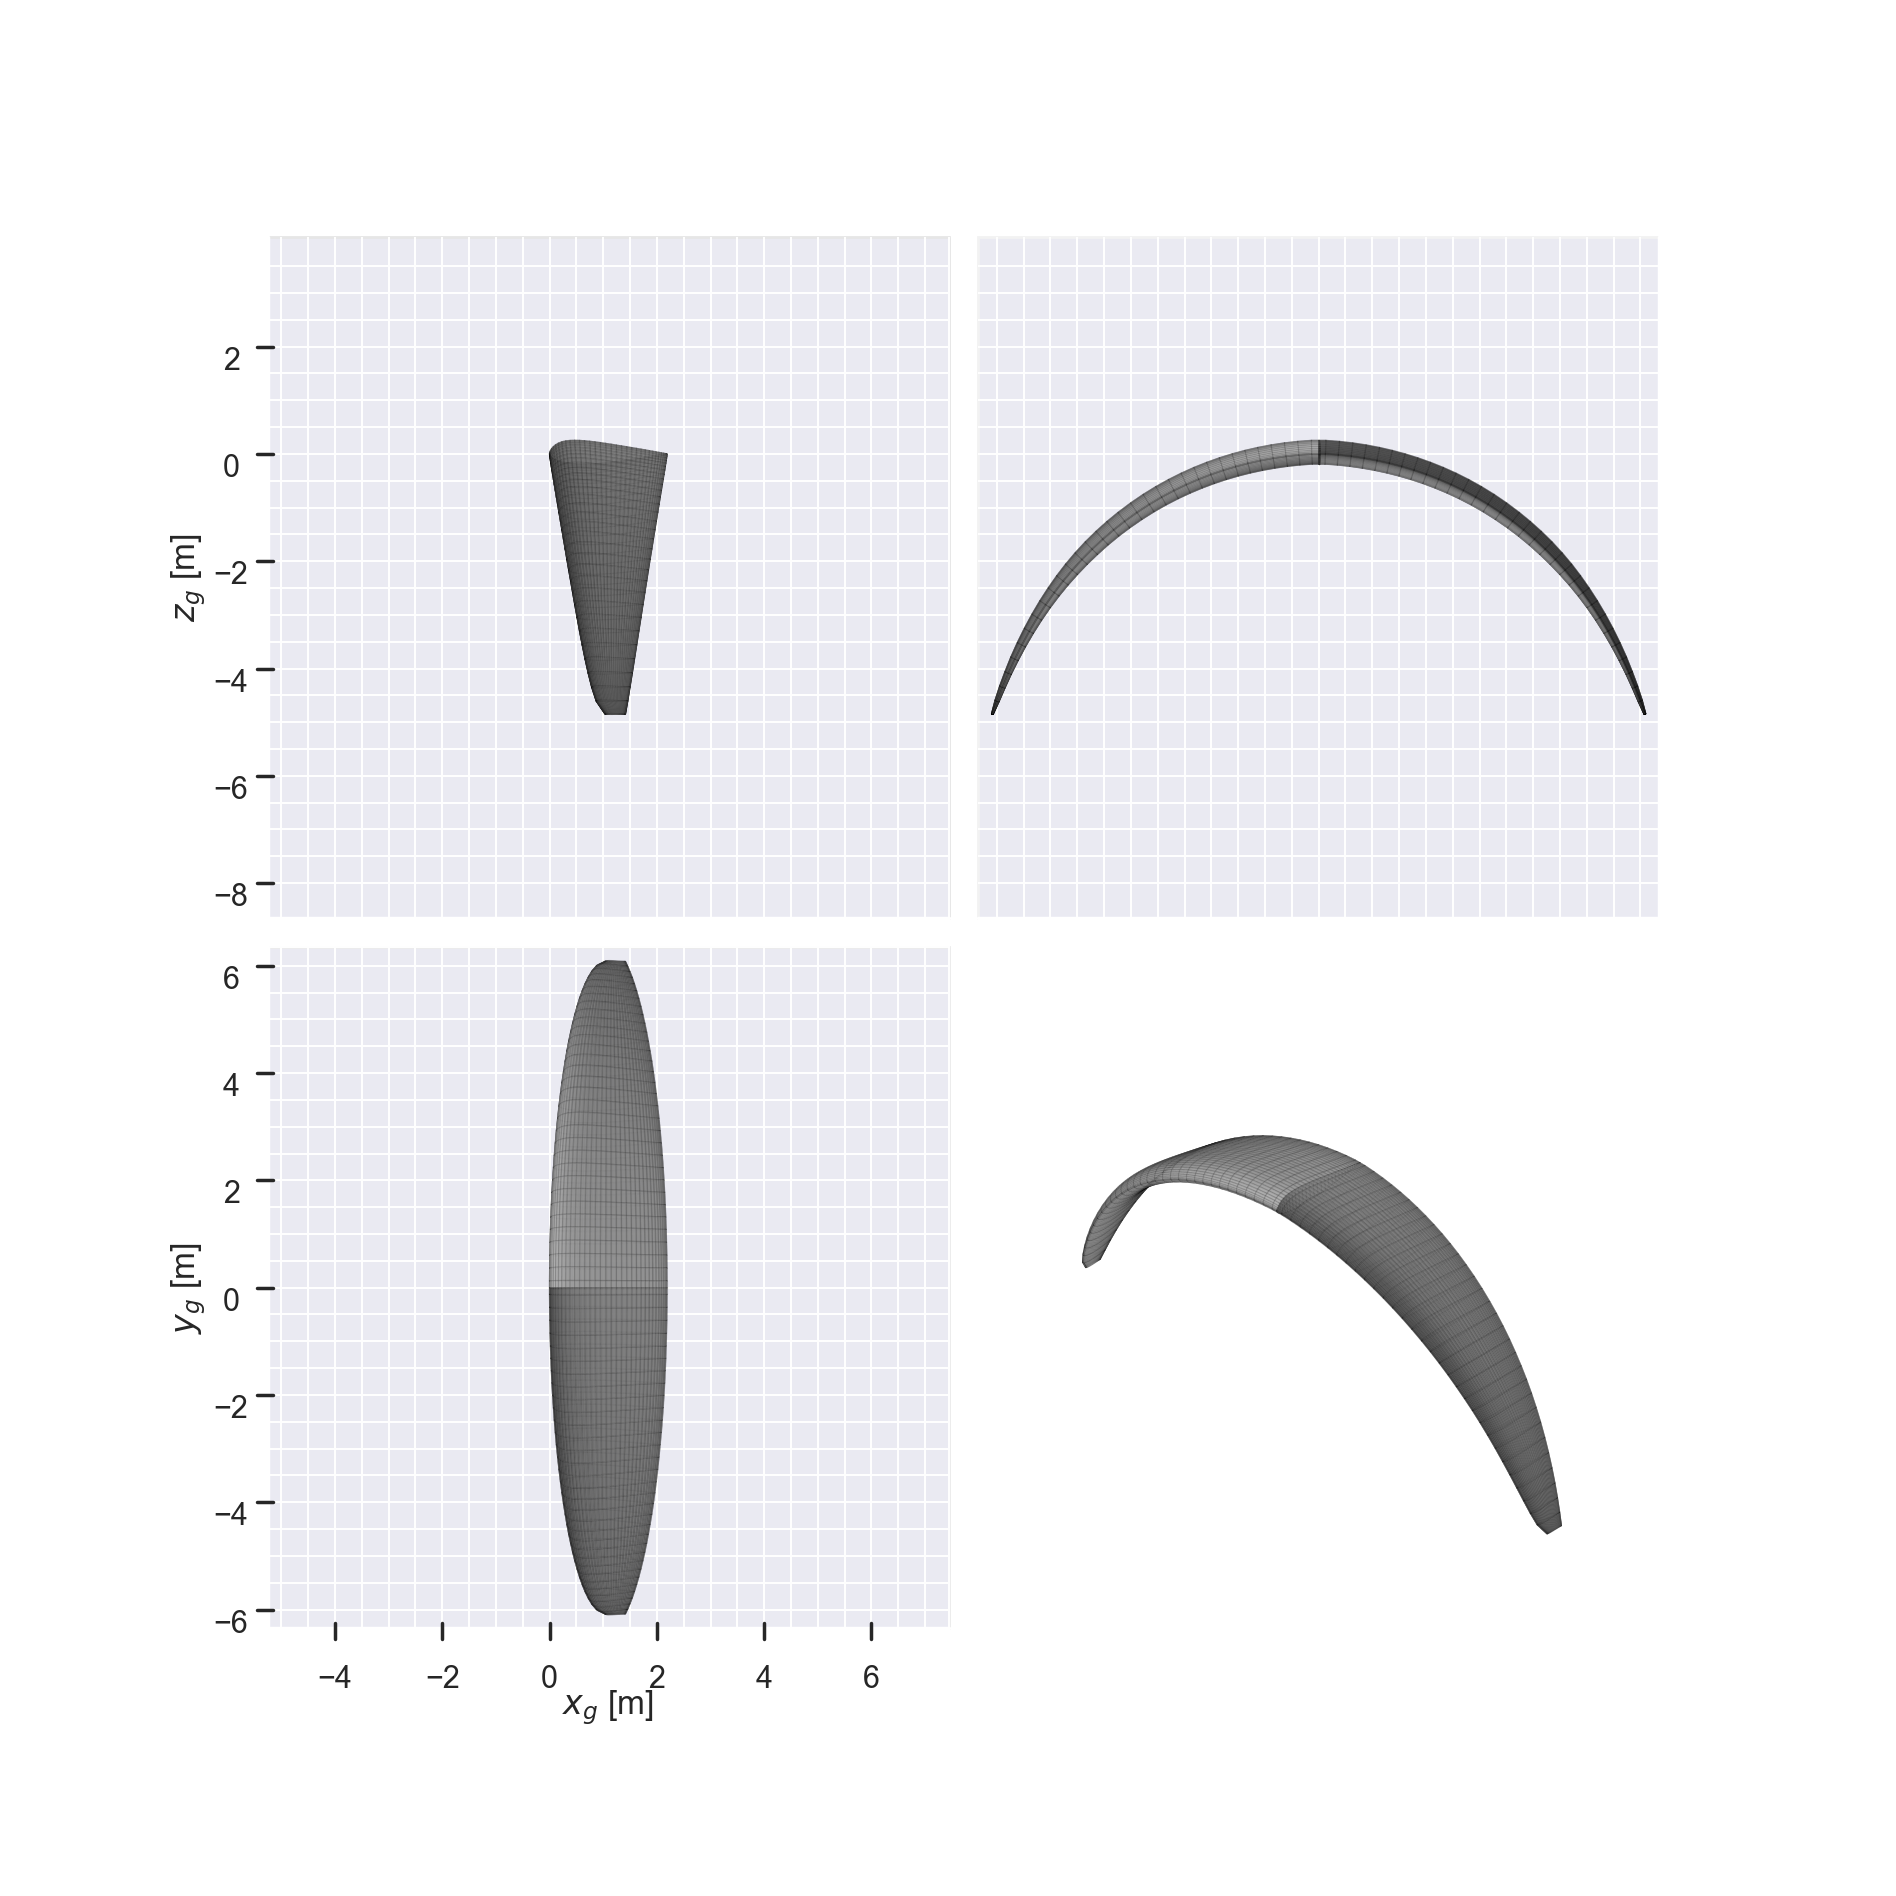
\includegraphics[width=1\linewidth]{figures/2D steady simulations/results/R1 V5 Satori 3 3D view.png}
    \caption{The R1 V5 Satori 3 3D view}
    \label{fig:The R1 V5 Satori 3 3D view}
\end{figure}

%%%%%%%%%%%%%%%%%%%%%%%%%%%%%%%%%%%% SUBSECTION 4

\subsection{The team rider feedbacks}
\label{sub:Ch1.6.4}

After several hours of adjustments and continuous use of the kite prototype until it reached its "final" shape (bearing in mind that the fabrics relax during the initial hours of testing), the team riders achieved higher Velocity Made Good (VMG) values upwind and maintained greater tether tension when going downwind. They enthusiastically declared that this kite was the most high-performing one they had ever tested and expressed optimism about the future of the kite we were developing.

Moreover, the accuracy in predicting kite performance and the alignment between theory and practice reassured the Ozone's design team about using science to shape their future kites. In fact, the kite surfing community has only recently embraced scientific knowledge in fluid mechanics, and these results served as Ozone's initial evidence of the value that numerical simulations can bring to the company.

It's important to note that many kites have benefited from my research on kite aerodynamics. This is because not all kites aim for the same performance characteristics. For instance, the smaller version of the R1 V5, which has an area of $11m^{2}$ compared to the $21m^{2}$ kite discussed in this report, is used in stronger winds where the emphasis is not on exploiting the finesse of the kite (as the wind is already strong, and other factors like the pilot's skill or the performance of the submerged foil in the water are limiting), but rather on its stability. As a result, the entirety of the work developed in this report has contributed to the development of this kite, which serves very different objectives, but for which the contribution of scientific research has proven to be beneficial. 

Once again, the feedback from the team riders during tests conducted on prototypes of these kites has proven to be in line with theory, and the kites developed in this manner have demonstrated higher performance than the existing ones.

%%%%%%%%%%%%%%%%%%%%%%%%%%%%%%%%%%%% Chapter Template

\chapter{Optimization} 	% Main chapter title
\label{Chapter2} 		% For referencing the chapter elsewhere, usage \ref{Chapter1}

%%%%%%%%%%%%%%%%%%%%%%%%%%%%%%%%%%%%

Following the design of the R1 V5 Satori 3 and discussions with the Ozone paragliding design team, my attention turned to enhancing the performance of the kite. To achieve this, I collaborated with Fred Pieri, a paraglider designer, to develop an optimization algorithm. This algorithm, written in Python, makes use of the Aerosandbox library.

%%%%%%%%%%%%%%%%%%%%%%%%%%%%%%%%%%%%%%%%%%%%%%%%%%%%%%%%%%%%%%%%%%%%%%%%%%%%%%%%
%%%%%%%%%%%%%%%%%%%%%%%%%%%%%%%%%%%% SECTION 1 %%%%%%%%%%%%%%%%%%%%%%%%%%%%%%%%%
%%%%%%%%%%%%%%%%%%%%%%%%%%%%%%%%%%%%%%%%%%%%%%%%%%%%%%%%%%%%%%%%%%%%%%%%%%%%%%%%

\section{Aerosandbox}
\label{sec:Ch2.1}

AeroSandbox\cite{aerosandbox} is a Python package that helps designing and optimizing aircrafts and other engineered systems. It is developed by Peter Sharpe, a graduate student studying aircraft design, multidisciplinary design optimization (MDO) and applied aerodynamics in MIT's Department of Aeronautics and Astronautics.

At its heart, AeroSandbox is an optimization suite that combines the ease-of-use of familiar NumPy syntax with the power of modern automatic differentiation.

This automatic differentiation dramatically improves optimization performance on large problems: design problems with tens of thousands of decision variables solve in seconds on a laptop. AeroSandbox also comes with dozens of end-to-end-differentiable aerospace physics models, allowing users to simultaneously optimize an aircraft's aerodynamics, structures, propulsion, mission trajectory, stability, and more.

%%%%%%%%%%%%%%%%%%%%%%%%%%%%%%%%%%%% SUBSECTION 1
\subsection{The 2D aerodynamics}
\label{sub:Ch2.1.1}

The 2D study uses \textbf{"NeuralFoil"}. It is a tool for rapid aerodynamics analysis of airfoils, similar to XFoil. Under the hood, NeuralFoil consists of physics-informed neural networks trained on tens of millions of XFoil runs.

NeuralFoil is 10 times faster than XFoil for a single analysis, and 1000 times faster for multipoint analysis, all with minimal loss in accuracy compared to XFoil. Due to the wide variety of training data and the embedding of several physics-based invariants, this accuracy is seen even on out-of-sample airfoils (i.e., airfoils it wasn't trained on). \cite{neuralfoil}

It uses the 2D Panel Method. It is a computational technique used in aerodynamics to analyze the flow of fluids around two-dimensional objects.
Here is a basic overview of how the 2D Panel Method works:
\begin{itemize}
    \item Discretization: The surface of the object is divided into a series of panels, which are typically flat or slightly curved. These panels represent small segments of the object's surface.
    \item Vortex Elements: Each panel is then modeled as a vortex element that produces a velocity field at its position. These elements create a mathematical representation of how the fluid interacts with the object's surface.
    \item Superposition Principle: The key idea behind the Panel Method is that the total velocity at any point in the flow field is the sum of the velocities induced by all the panels. This is based on the principle of superposition, which allows you to add up the effects of individual panels to obtain the overall flow field.
    \item Kutta Condition: To ensure the accuracy of the method, a condition called the Kutta condition is applied at the trailing edge of the airfoil. This condition ensures that the flow separates smoothly from the trailing edge, which is physically realistic. (i.e. the flow circulation is conserved).
    \item Computational Solution: The method involves solving a system of linear equations to satisfy the boundary conditions at the surface of the object (normal velocity is equal to zero) and the Kutta condition at the trailing edge. Once this system is solved, it provides the velocity distribution around the object and can be used to calculate various aerodynamic parameters such as lift, drag, and pressure distribution.
\end{itemize}

The 2D Panel Method is especially useful for preliminary design and analysis. While it simplifies certain aspects of fluid dynamics, it can provide valuable insights and accurate results for many practical engineering applications.

%%%%%%%%%%%%%%%%%%%%%%%%%%%%%%%%%%%% SUBSECTION 2
\subsection{The 3D aerodynamics}
\label{sub:Ch2.1.2}

The 3D study uses the \textbf{"Vortex Lattice Mathod (VLM)"}. It is a simplified mathematical approach that provides an approximate solution to the flow field around these objects. VLM is particularly useful for low-speed and subsonic aerodynamic analyses. Here is a basic overview of how the Vortex Lattice Method works:
\begin{itemize}
    \item Discretization: The surface of the aerodynamic object is divided into a set of smaller, interconnected panels or segments. These panels are often assumed to be flat and have a constant strength vortex associated with them.
    \item Vortex Representation: Each panel generates a vortex, and these vortices collectively form a lattice that represents the overall geometry of the object. The strength and location of these vortices are determined based on the local flow conditions and geometry.
    \item Induced Velocities: The induced velocity at any point in the flow field, caused by all the vortices in the lattice, is calculated using mathematical equations. This induced velocity represents how the vortices affect the flow at a particular location.
    \item Boundary Conditions: The VLM considers boundary conditions, such as the no-slip condition at the object's surface and the freestream velocity far from the object.
    \item Solution for Aerodynamic Forces: Using the induced velocities and boundary conditions, the method calculates aerodynamic forces and moments on the object, such as lift, drag, and pitch moment.
\end{itemize}

It's important to note that the Vortex Lattice Method is a simplified approach and comes with certain limitations. For instance, it assumes steady, incompressible, and inviscid flow, neglecting turbulence effects and compressibility. As such, it is most suitable for preliminary design and analysis where a quick assessment of an object's aerodynamic characteristics is needed. Despite its simplifications, the Vortex Lattice Method has been widely used in the early stages of aircraft design and in the analysis of various aerodynamic configurations due to its efficiency and ability to provide valuable insights into the behavior of aerodynamic systems.

Note that Aerosandbox also offers to use the \textbf{"Lifting Line Theory"} (LLT). It is a more advanced analytical method than the VLM used to calculate the lift distribution along the span of a finite wing. It considers the variation in lift across the wing, taking into account the effects of downwash and induced drag. The LLT relies on the concept of vortex filaments to model the lift distribution and uses integral equations to determine the lift characteristics of the wing.

%%%%%%%%%%%%%%%%%%%%%%%%%%%%%%%%%%%% SUBSECTION 3
\subsection{The geometry}
\label{sub:Ch2.1.3}

The three main geometry objects used in this study are the "Airplane", the "Airfoil" and the "Kulfan Airfoil".

\begin{itemize}
    \item The Airplane : it encapsulates the entire aircraft, comprising a collection of "Wing" objects, which constitute integral parts of the aircraft and are described by a list of sections, each featuring position, airfoil, twist angle, and chord parameters. Additionally, there is a list of "Fuselage" objects, which are also integral components of the aircraft and are associated with reference values.
    \item The Airfoil : It can be defined using either a set of coordinates or a NACA airfoil.
    \item The Kulfan Airfoil : the class shape transformation (CST) (Kulfan, 2008) is a popular airfoil parameterization \cite{Kulfan}.It generates a shape using Bernstein polynomials to scale a class function, which is most often a base airfoil shape. They are built with "lower weights" (8 points), "upper weights" (8 points), "leading edge weight" (1 point) and a trailing edge thickness. This class has recently been added (August 2023) to Aerosandbox in order to allow 2D airfoil optimization.   
\end{itemize}

%%%%%%%%%%%%%%%%%%%%%%%%%%%%%%%%%%%% SUBSECTION 4
\subsection{The optimization}
\label{sub:Ch2.1.4}

The Aerosandbox optimization part uses \textbf{"CasADi"}, an open-source software tool for numerical optimization in general and optimal control (i.e. optimization involving differential equations) in particular \cite{Andersson2018}. It solves the optimization problems using CasADi with IPOPT backend. 

\textbf{"Interior Point OPTimizer, pronounced I-P-Opt"} (IPOPT) is a software library for large scale nonlinear optimization of continuous systems \cite{ipopt}. IPOPT implements a \textbf{primal-dual interior point method}, and uses line searches based on Filter methods (Fletcher and Leyffer).

Primal-dual interior point method has the advantages of :
\begin{itemize}
    \item efficiency for large-scale problems (can handle problems with a large number of variables and constraints)
    \item global convergence (can find solutions that are globally optimal or nearly optimal) 
    \item handling inequality constraints
    \item well-suited for linear and convex problems
    \item predictable convergence behavior
\end{itemize}

but also has the disadvantages of :
\begin{itemize}
    \item lack of flexibility (primarily designed for convex optimization problems)
    \item sensitivity to initial conditions
    \item computational cost
    \item limited support for non-smooth functions (functions that have continuous derivatives of all orders)
\end{itemize}

Consequently, although certain drawbacks, such as computational cost and sensitivity to initial conditions, were encountered in its utilization, the primal-dual interior point method continued to prove highly suitable for this specific application.


% Here is a basic overview of how the \textbf{primal-dual interior point method} works :

% Starting from a nonlinear optimization problem with inequality constraints:
% \begin{equation}
%     \left\{
%     \begin{array}{ll}
%         minimize & f(x) \\
%         subject\: to & x \in \mathbf{R}^{N} \\
%         & c_{i}(x) \geq 0, for\: i=1,...,m \\
%         where & f:\mathbf{R}^{N} \rightarrow \mathbf{R}, c_{i}:\mathbf{R}^{N} \rightarrow \mathbf{R}
%     \end{array}
% \right.
% \label{eq:non linear optimization problem}
% \end{equation}

% The primal-dual interior point method solves an inequality-constrained optimization problem by converting it into an unconstrained objective function whose minimum we hope to find efficiently. Specifically, the logarithmic barrier function associated with \ref{eq:non linear optimization problem} is :
% \begin{equation}
%     B(x,\mu) = f(x) - \mu \sum_{i=1}^{m} log(c_{i}(x))
% \label{eq:logarithmic barrier function}
% \end{equation}

% Then, using the gradient of the barrier function and, in addition to the original ("primal") variable x, introducing a Lagrange multiplier-inspired dual variable $\lambda \in \mathbf{R}^{m}$ :
% \begin{equation}
%     c_{i}(x) \lambda _{i} = \mu, \forall i =1,...,m
%     \label{eq:Lagrange multiplier-inspired dual variable}
% \end{equation}
% we try to find the $(x_{\mu}, \lambda_{\mu})$ for which the gradient of the barrier function is zero.

% We get an equation for the gradient : 
% \begin{equation}
%     \nabla B(x_{\mu}), \lambda_{\mu} = \nabla f(x_{\mu}) - \mu \sum_{i=1}^{m} \frac{1}{c_{i}(x_{\mu})} \nabla c_{i}(x_{\mu}) = \nabla f(x_{\mu}) - J(x_{\mu})^{T} \lambda_{\mu} = 0
%     \label{eq:equation for the gradient}
% \end{equation}

% where the matrix J is the Jacobian of the constraints c(x).

% The intuition behind \ref{eq:equation for the gradient} is that the gradient of f(x) should lie in the subspace spanned by the constraints' gradients. The "perturbed complementarity" \ref{eq:Lagrange multiplier-inspired dual variable} with small $\mu$  can be understood as the condition that the solution should either lie near the boundary $c_{i}(x) = 0$, or that the projection of the gradient $\nabla f$ on the constraint component $c_{i}(x)$ normal should be almost zero.

% Applying Newton's method to \ref{eq:Lagrange multiplier-inspired dual variable} and \ref{eq:equation for the gradient}, we get the equation where appear H, the Hessian matrix of $B(x,\mu)$ and diag(), diagonal matrices : 
% \begin{equation}
%     \begin{pmatrix}
%         H(x,\lambda) & -J(x)^{T}\\
%         diag(\lambda)J(x) & diag(c(x))
%     \end{pmatrix}
%     \begin{pmatrix}
%         p_{x}\\
%         p_{\lambda}
%     \end{pmatrix} = 
%     \begin{pmatrix}
%         -\nabla f(x) + J(x)^{T} \lambda\\
%         \mu - diag(c(x))\lambda
%     \end{pmatrix}
%     \label{eq:equation for the search direction for iteratively updating }
% \end{equation}  

% Here, $(p_{x},p_{\lambda})$ is the search direction for iteratively updating $(x, \lambda)$.

% Because of \ref{eq:non linear optimization problem} and \ref{eq:Lagrange multiplier-inspired dual variable} the condition $\lambda \geq 0$ should be enforced at each step. This can be done by choosing appropriate $\alpha$ : 
% $(x, \lambda) \rightarrow (x+\alpha p_{x}, \lambda + \alpha p_{\lambda})$

%%%%%%%%%%%%%%%%%%%%%%%%%%%%%%%%%%%%%%%%%%%%%%%%%%%%%%%%%%%%%%%%%%%%%%%%%%%%%%%%
%%%%%%%%%%%%%%%%%%%%%%%%%%%%%%%%%%%% SECTION 2 %%%%%%%%%%%%%%%%%%%%%%%%%%%%%%%%%
%%%%%%%%%%%%%%%%%%%%%%%%%%%%%%%%%%%%%%%%%%%%%%%%%%%%%%%%%%%%%%%%%%%%%%%%%%%%%%%%

\section{2D optimization}
\label{sec:Ch2.2}

The 2D optimization algorithm was developed with the objective of improving the airfoil profile beyond that of the R1 V5 Satori 3, starting with the same base profile and introducing variations to the four parameters on the upper surface. The decision was made to retain the lower surface of the R1 V5 Satori 3 since it exhibited a "realistic" shape that yielded favorable results. The optimization program in Python incorporated the following conditions : 
\begin{itemize}
    \item The Cl must stay superior to the initial airfoil ones at few angles of attack ( 0°, 2.5°, 5°, 7.5°, 10°, 12.5°, 15°)
    \item The trailing edge angle must be superior or equal to the initial airfoil one
    \item The local thickness must stay positive
    \item The $\frac{d^{2}}{d^{2}_{x}}$ of the local thickness must stay negative
    \item The $\frac{d^{2}}{d^{2}_{x}}$ of the local camber must stay negative
    \item The $\frac{d}{d_{x}}$ of the upper coordinates must stay negative after the upper apex
    \item The $\frac{d}{d_{x}}$ of the lower coordinates must stay positive after the lower apex
    \item the maximum thickness must be superior or equal to 19\% of the chord
\end{itemize}

The following result was reached after 4 secondes :
\begin{figure}[H]
    \centering
    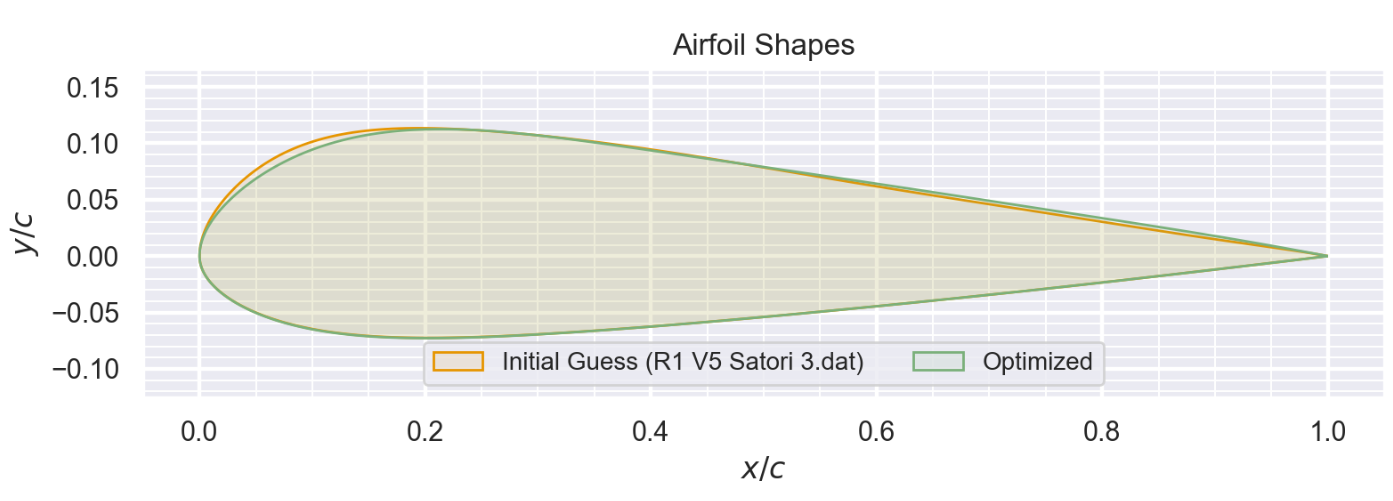
\includegraphics[width=1.\textwidth]{figures/Optimization/2D/Comparison intial guess and optimized airfoils.png}
    \caption{Comparison between the Initial Guess Airfoil and the Optimized Airfoil}
    \label{fig:Comparison between the Initial Guess Airfoil and the Optimized Airfoil}
\end{figure}

We can see on the figure \ref{fig:Comparison between the Initial Guess Airfoil and the Optimized Airfoil} that the algorithm put the apex slightly backward to increase the airfoil finesse.

As a results, simulations with Fluent were run in order to validate the airfoil before starting a new prototype : 

\begin{figure}[H]
    \centering
    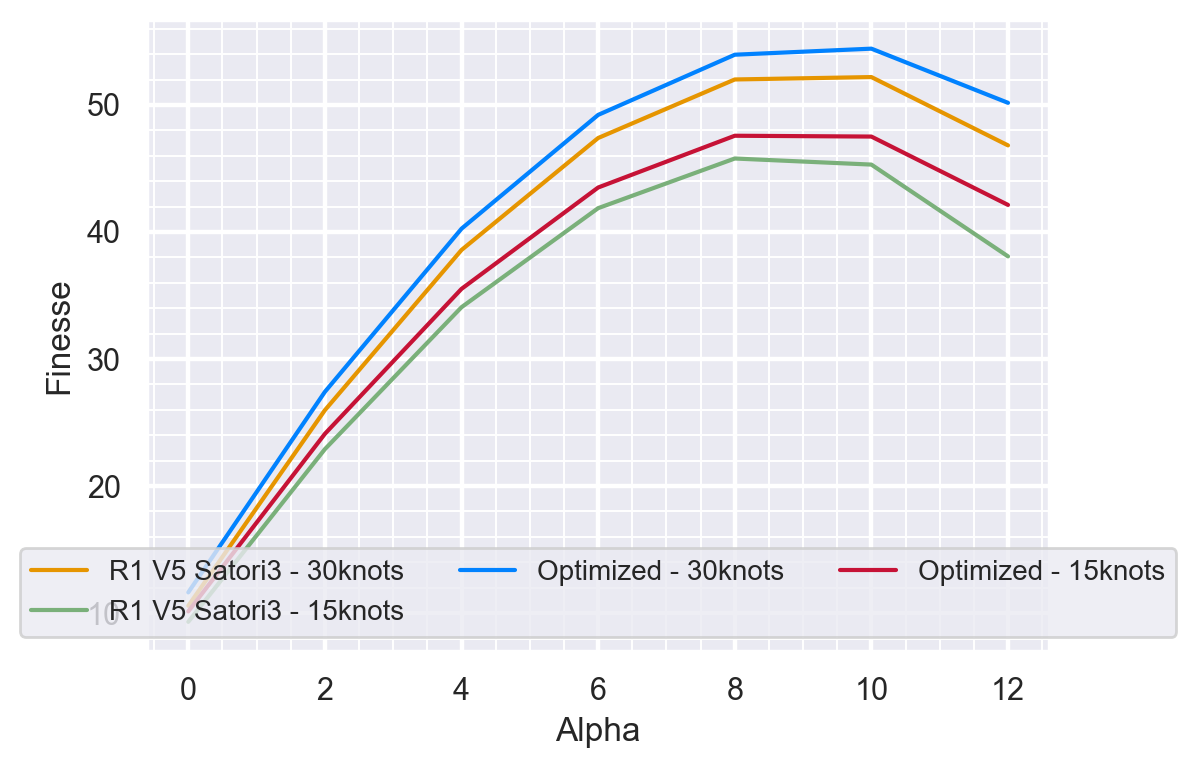
\includegraphics[width=1.\textwidth]{figures/Optimization/2D/finesse optimized and Satori3.png}
    \caption{Finesses of the R1 V5 Satori3 and the optimized airfoils (FLUENT)}
    \label{fig:Finesses of the R1 V5 Satori3 and the optimized airfoils}
\end{figure}

Figure \ref{fig:Finesses of the R1 V5 Satori3 and the optimized airfoils} suggests that the theoretically optimized airfoil should outperform the R1 V5 Satori 3. 

It's worth noting that 3D effects and actual testing may reveal unforeseen factors that could potentially impact the performance of the optimized profile. However, at this stage, there is confidence that this airfoil is an improvement over the current airfoil under evaluation.


%%%%%%%%%%%%%%%%%%%%%%%%%%%%%%%%%%%%%%%%%%%%%%%%%%%%%%%%%%%%%%%%%%%%%%%%%%%%%%%%
%%%%%%%%%%%%%%%%%%%%%%%%%%%%%%%%%%%% SECTION 3 %%%%%%%%%%%%%%%%%%%%%%%%%%%%%%%%%
%%%%%%%%%%%%%%%%%%%%%%%%%%%%%%%%%%%%%%%%%%%%%%%%%%%%%%%%%%%%%%%%%%%%%%%%%%%%%%%%

\section{3D optimization}
\label{sec:Ch2.3}

An alternative approach to enhance the performance of the R1 involves optimizing 3D parameters. I initially concentrated on optimizing the twist distribution along the span and subsequently extended the optimization to the wing's planform. 

The primary challenge associated with 3D optimization lies in the computational cost. In practice, even though VLM simulations might not appear significantly more complex at first glance, the algorithm must address 33 variables in 3D (corresponding to 33 sections along the wing's span) as opposed to the 10 variables used in 2D (related to Kulfan airfoil parameters).

This elevated level of complexity may result in outcomes that fail to converge, an excessive number of iterations, or a shortage of available computer memory space.

Additionally, the need for spatial discretization along both the wing's span and its chord required an evaluation of spatial convergence when employing the vortex lattice method before initiating the optimization of the twist distribution along the span.

\begin{figure}[H]
    \centering
    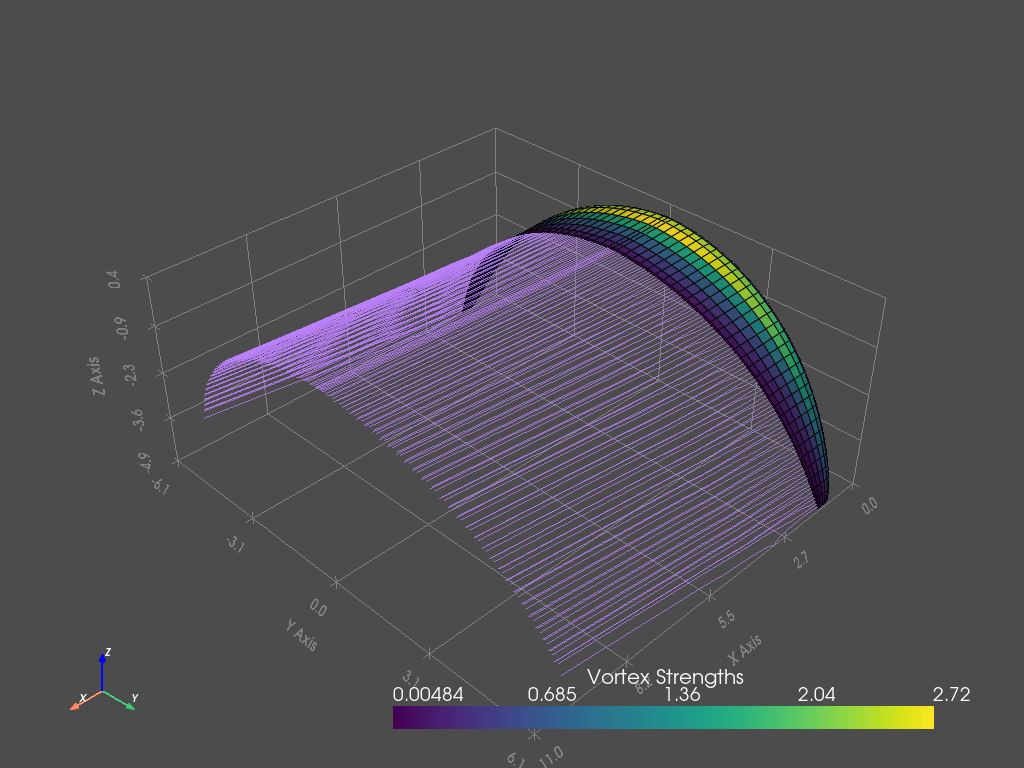
\includegraphics[width=1.\linewidth]{figures/Optimization/3D/vlm.png}
    \caption{Draw of a VLM simulation on the R1 V5 Satori 3}
    \label{fig:Draw of a VLM simulation on the R1 V5 Satori 3}
\end{figure}

%%%%%%%%%%%%%%%%%%%%%%%%%%%%%%%%%%%% SUBSECTION 1
\subsection{The spatial convergence of the VLM simulations}
\label{sub:Ch2.3.1}

Aerosandbox offers to discretize along the chord via $"chordwise\_resolution"$ and along the span via $"spanwise\_resolution"$, two parameters of the VLM function. Note that $spanwise\_resolution$ is the number of element aerosandbox considers between two sections of the wings. As the wing is defined with 33 sections, a $spanwise\_resolution$ of k means $33 * k$ elements along the span.

Therefore, VLM simulations have been run for different values of these very two parameters in order to find the values for which the simulations can be considered to have sufficiently converged to their asymptotic values.

Note that results in terms of relative error don't change with the speed or the aerodynamic coefficient we calculate.

\begin{figure}[H]
    \centering
    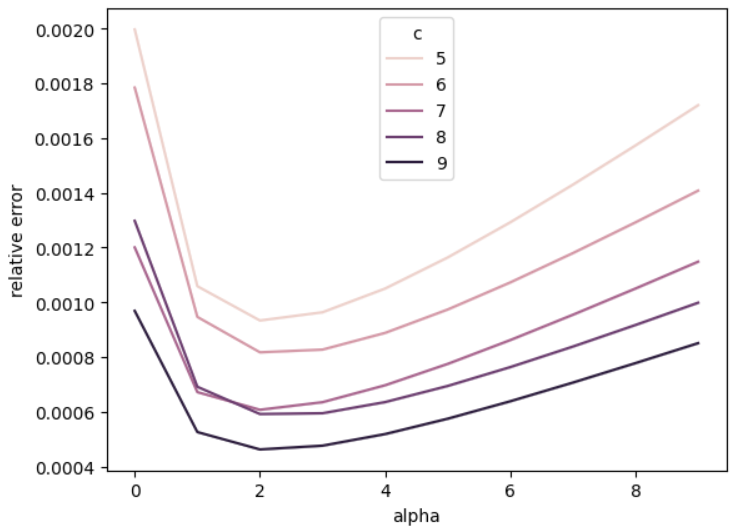
\includegraphics[width=0.8\textwidth]{figures/Optimization/3D/error_span_1_2.png}
    \caption{Relative error in lift force between a spanwise resolution of 1 and 2}
    \label{fig:Relative error in lift force between a spanwise resolution of 1 and 2}
\end{figure}

The figure \ref{fig:Relative error in lift force between a spanwise resolution of 1 and 2} shows that choosing $spanwise\_resolution = 1$ is enough to consider the simulation to have spatially converged. Note that in figures  \ref{fig:Relative error in lift force between a spanwise resolution of 1 and 2} and \ref{fig:Relative error in lift force} "c" is the $chordwise\_resolution$ parameter and "s" is the $spanwise\_resolution$ parameter.

\begin{figure}[H]
    \begin{subfigure}{0.5\textwidth}
    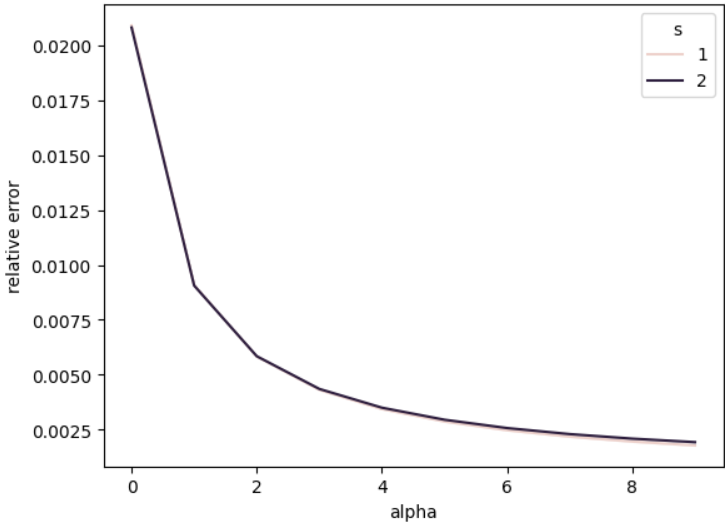
\includegraphics[width=1.\textwidth]{figures/Optimization/3D/error_chord_7_8.png}
    \caption{between chordwise resolutions of 7 and 8}
    \label{fig:between chordwise resolutions of 7 and 8}
    \end{subfigure}
    \begin{subfigure}{0.5\textwidth}
    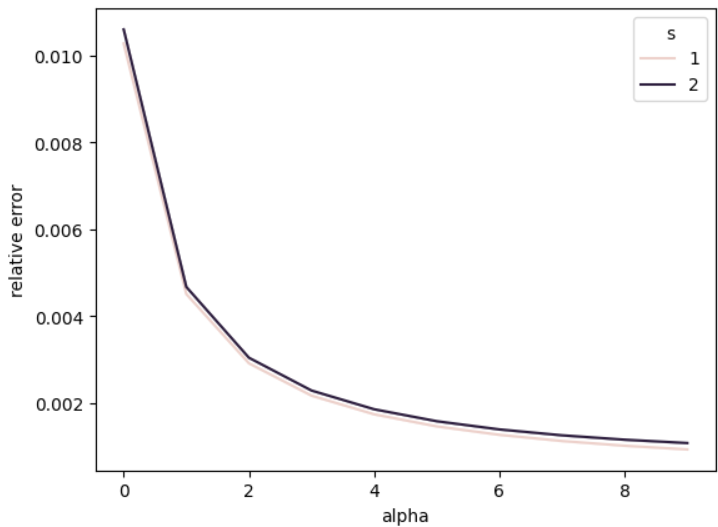
\includegraphics[width=1.\textwidth]{figures/Optimization/3D/error_chord_8_9.png}
    \caption{between chordwise resolutions of 8 and 9}
    \label{fig:between chordwise resolutions of 8 and 9}
    \end{subfigure}
    \caption{Relative error in lift force}
\label{fig:Relative error in lift force}
\end{figure}

The figure \ref{fig:Relative error in lift force} shows that we can already consider the VLM simulations to have converged for $chordwise\_resolution = 8$. This $chordwise\_resolution$ value is a good compromise between computational cost and accuracy.

\textbf{As a consequence, the following parameters have been selected for VLM simulations using Aerosandbox to achieve spatial convergence while minimizing computational costs : }
\begin{itemize}
    \item $chordwise\_resolution = 8$
    \item $spanwise\_resolution = 1$
\end{itemize}

%%%%%%%%%%%%%%%%%%%%%%%%%%%%%%%%%%%% SUBSECTION 2
\subsection{The twist optimization}
\label{sub:Ch2.3.2}

The twist optimization is intended to address the issue of reduced finesse at high angles of attack and during downwind maneuvers. Based on feedback from team riders, the existing kites do not exhibit sufficient forward flight characteristics, resulting in riders experiencing a lack of tension in the lines during their rides. Furthermore, Benoit Augier, a Ph.D. expert in fluid mechanics at the Marine Hydrodynamic Laboratory in Brest, who is currently collaborating with the French kitesurfing team for the Olympic Games, suggests that there is still room for reducing kite drag under these conditions changing the kite twist or its planform.

However, it encounters a challenge in terms of computational complexity. Unlike 2D optimizations, which typically take about 10 minutes to complete, the twist optimization algorithm requires several hours to run. If I lack the resources required to conduct simulations until we have a precise law that defines the optimal kite twist at various angles of attack, I can, however, run a simulation at a single angle of attack to obtain an initial glimpse of what such a twist profile might look like.

Therefore, I executed the optimization algorithm at a 9° angle of attack and a wind speed of 20 knots, under the following conditions :

\begin{itemize}
    \item The kite should support a load of 150 kg
    \item The $\frac{d}{d_{z}}$ of the twist cannot exceed 3°/section (a physical constraint that ensures manufacturability)
\end{itemize}

The algorithm required 62 minutes to complete.

\begin{figure}[H]
    \centering
    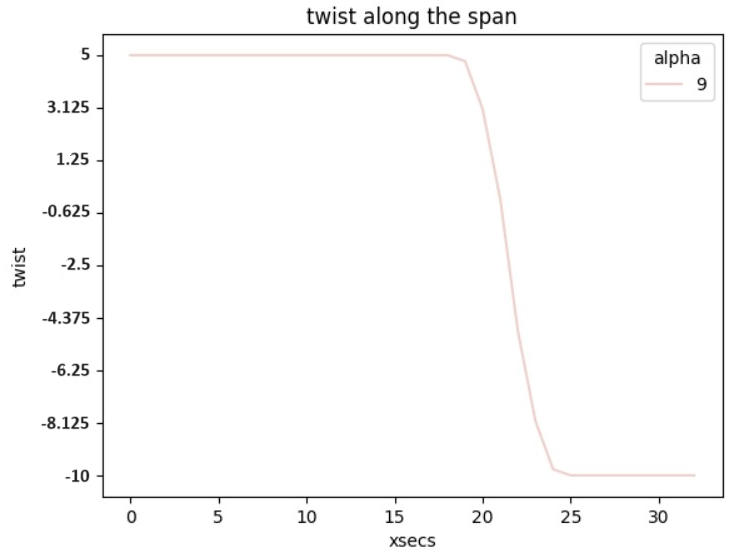
\includegraphics[width=0.7\textwidth]{figures/Optimization/3D/twist along the span.png}
    \caption{The twist distribution along the wing's span that minimizes drag at a 9° angle of attack during downwind conditions (at 20 knots)}
    \label{fig:Result of the twist law along the span the gives the minimum drag at 9° in downwind conditions (20 knots)}
\end{figure}

The figure \ref{fig:Result of the twist law along the span the gives the minimum drag at 9° in downwind conditions (20 knots)} indicates that the algorithm strives to distribute the load evenly across the kite's middle section and minimize drag resulting from tip vortices. 

Currently, these results haven't been utilized by Ozone kitesurf due to the tight deadlines the brand faces for submitting the kite sail design for the 2028 Olympic Games. However, this 3D optimization algorithm could prove beneficial for the brand if tested on their future prototypes, offering an alternative means of improving kites performances.

Furthermore, the Ozone paraglider design team is already engaged in this project, and their upcoming paraglider design may benefit from the use of this algorithm.

While planform optimization has also been implemented, it is computationally intensive and strains the capabilities of my computer. With access to more powerful computing resources, both planform and twist optimizations could be conducted simultaneously, providing the design team with a kite that fully harnesses the potential of its airfoil.

%%%%%%%%%%%%%%%%%%%%%%%%%%%%%%%%%%%% SUBSECTION 3
\subsection{The equilibrium of moments}
\label{sub:Ch2.3.3}

Another algorithm has been employed for the prediction of the kite's position within the wind window. By leveraging the knowledge of the bar position set by the athlete and applying the principles of moment equilibrium (minimizing the absolute value of the moment with an optimization algorithm) around the athlete between the kite's aerodynamic forces and the drag in the lines, we were able to compute the kite's angle of attack.

Remarkably, this algorithm achieved a prediction that had previously remained elusive for Ozone and, as far as my research indicates, for anyone in the kitesurfing community: the angle of attack of a kite and its positioning in the wind window, relying solely on the kite's aerodynamic properties without knowledge of water foil drag or athlete drag.

Consequently, the algorithm effectively validated the data in Table \ref{tab:commonly_accepted_inlet_values} and stands as a robust tool for Ozone to forecast kite flight conditions based on the athlete's speed.

\begin{figure}[H]
    \centering
    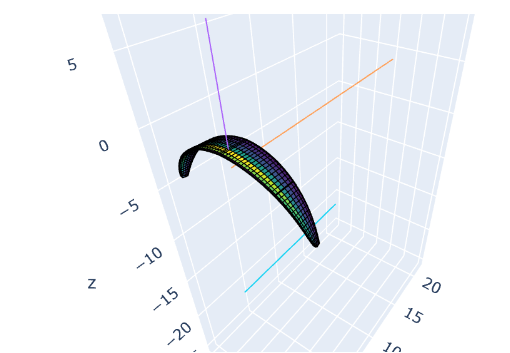
\includegraphics[width=1.\linewidth]{figures/Optimization/3D/equilibre moment.png}
    \caption{An illustration depicting the equilibrium of moments on the athlete (25 meters under the kite) (with rescaled forces)}
    \label{fig:An illustration depicting the equilibrium of moments}
\end{figure}

\begin{figure}[H]
  \begin{subfigure}{0.5\textwidth}
    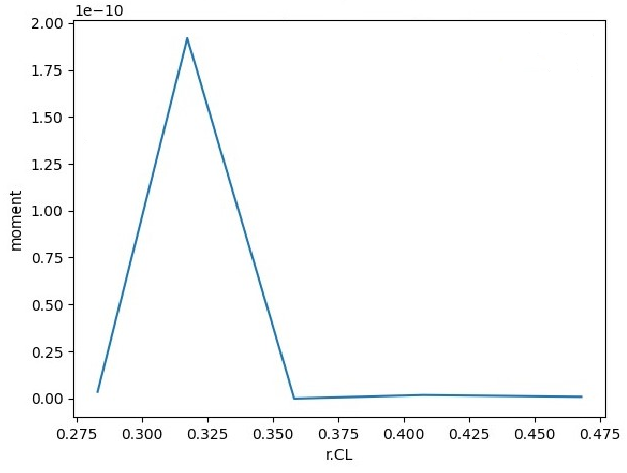
\includegraphics[width=\textwidth]{figures/Optimization/3D/moment equilibre.png}
    \caption{Moment (Nm) against Cl}
  \end{subfigure}
  \begin{subfigure}{0.5\textwidth}
    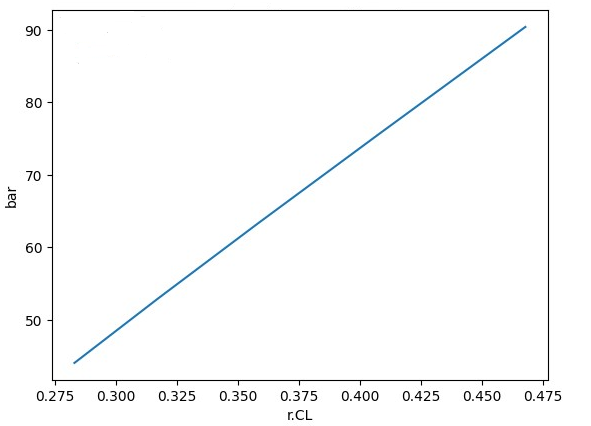
\includegraphics[width=\textwidth]{figures/Optimization/3D/moment equilibre bar.png}
    \caption{Bar position (cm) against Cl}
  \end{subfigure}
  \begin{subfigure}{0.5\textwidth}
    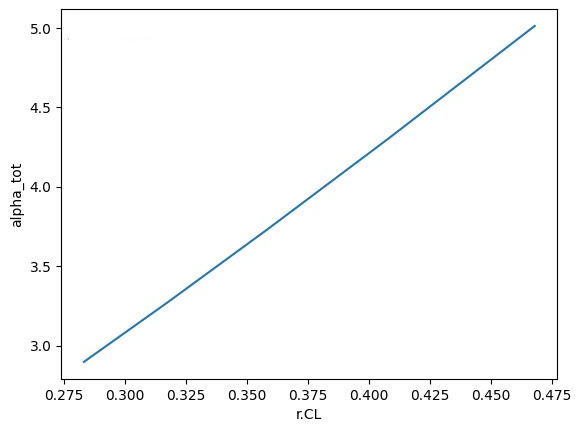
\includegraphics[width=\textwidth]{figures/Optimization/3D/moment equilibre alpha.png}
    \caption{Angle of attack (°) against Cl}
  \end{subfigure}
  \caption{Plots at 35 knots (Upwind conditions)}
  \label{Plots at 35 knots (Upwind conditions)}
\end{figure}

The information presented in Figure \ref{Plots at 35 knots (Upwind conditions)} clearly indicates that, under upwind conditions, and with an offset applied to the bar position to attain the actual kite deformation, the kite's angle of attack falls within the range of 0° to 5°, aligning with the predictions detailed in Table \ref{tab:commonly_accepted_inlet_values}.
%%%%%%%%%%%%%%%%%%%%%%%%%%%%%%%%%%%% Chapter Template

\chapter{Stability} 	% Main chapter title
\label{Chapter3} 		% For referencing the chapter elsewhere, usage \ref{Chapter1}

%%%%%%%%%%%%%%%%%%%%%%%%%%%%%%%%%%%%

During discussions with the team riders testing the new prototypes, it became evident that another critical phenomenon significantly impacted kite performance. 

In general, when a rider is moving downwind, they prefer the kite to exhibit a strong forward impulse, causing it to move deep into the wind window, even if the athlete maintains bar tension. Conversely, when a rider is heading upwind, the kite naturally wants to surge forward, especially when it flies at high Reynolds numbers and low angles of attack. But in contrast to downwind conditions, when the kite surges forward while going upwind, it tends to move out of the wind window. When the brakes halt the kite's forward movement after "shooting" forward, if the kite continues to progress forward due to a negative pitching moment, it may collapse. 

The manner in which a kite behaves when coming to a stop after moving forward, and how it attains its moment equilibrium, is frequently referred to as \textbf{"stability"} in kitesurfing. An unstable kite is one that continues to move forward even after the brakes have stopped it during a "shoot" (dynamic forward flight); it is a kite that proves challenging, and at times impossible, to control because it \textbf{collapses}.







\begin{figure}[H]
    \centering
    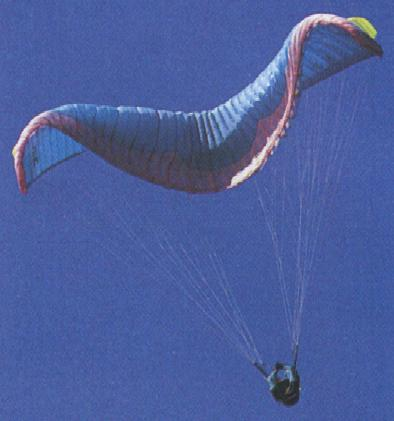
\includegraphics[width = 0.5\linewidth]{figures/Stability/front collapse.jpg}
    \caption{Picture of a paraglider pilot experiencing a front collapse}
    \label{fig:Picture of a paraglider pilot experiencing a front collapse}
\end{figure}


%%%%%%%%%%%%%%%%%%%%%%%%%%%%%%%%%%%%%%%%%%%%%%%%%%%%%%%%%%%%%%%%%%%%%%%%%%%%%%%%
%%%%%%%%%%%%%%%%%%%%%%%%%%%%%%%%%%%% SECTION 1 %%%%%%%%%%%%%%%%%%%%%%%%%%%%%%%%%
%%%%%%%%%%%%%%%%%%%%%%%%%%%%%%%%%%%%%%%%%%%%%%%%%%%%%%%%%%%%%%%%%%%%%%%%%%%%%%%%

\section{The aerodynamic definition of stability}
\label{sec:Ch3.1}

This issue of stability is well known in the paragliding world. As the physics is quite the same and the stakes are much higher, the Ozone paragliders designers have been able to help me translating the notion of stability in terms of aerodynamics. 

Contrary to the popular belief, a kite doesn't collapse when its incidence becomes negative, but before. "the collapse comes from the fact that the A lines bend more than the B lines under their own aerodynamic drag", according to the Ozone paraglider designers. \\

\begin{wrapfigure}{r}{0.5\textwidth}
\centering
    \includegraphics[width=0.4\textwidth]{figures/Stability/Schéma AB.png}
    \caption{A lines, B lines and lift on a kite airfoil}
    \label{fig:A lines, B lines and lift on an airfoil}
\end{wrapfigure}
Assuming that A lines drag and B lines drag are the same, for the kite to be stable, the tension in the A lines must be higher than the tension in the B lines. It also means that the aerodynamic force component collinear with the lines must be higher in the A lines than the B lines.\\

% \vspace{0.5cm}
Assuming that A lines and B lines are parallels near their towpoints (where the kite lines are tied) and considering a LIFT that represents the aerodynamic force component collinear with the lines, we have : 

\begin{figure}[H]
\centering
    \includegraphics[width=0.9\textwidth]{figures/Stability/schéma tension AB.png}
    \caption{A and B tensions on a kite airfoil}
    \label{fig:A and B tensions on a kite airfoil}
\end{figure}

\begin{equation}
\left \{
    \begin{array}{r c l}
        T_{A} = LIFT \frac{X_{B} - X_{cp}}{X_{B} - X_{A}} \\
        T_{B} = LIFT \frac{X_{cp} - X_{A}}{X_{B} - X_{A}} 
    \end{array}
    \right .
   \label{tension AB}
\end{equation}

\begin{equation}
    T_{A} \geq T_{B}M_{S} \iff X_{cp} \leq  \frac{X_{B}+X_{A}}{2M_{S}}
    \label{eq:last equation}
\end{equation}

With $M_{S}$ the static margin.

\textbf{As a result, we understand here that the aerodynamic force position along the chord Xcp is a measure of the kite stability}.\\


%%%%%%%%%%%%%%%%%%%%%%%%%%%%%%%%%%%%%%%%%%%%%%%%%%%%%%%%%%%%%%%%%%%%%%%%%%%%%%%%
%%%%%%%%%%%%%%%%%%%%%%%%%%%%%%%%%%%% SECTION 3 %%%%%%%%%%%%%%%%%%%%%%%%%%%%%%%%%
%%%%%%%%%%%%%%%%%%%%%%%%%%%%%%%%%%%%%%%%%%%%%%%%%%%%%%%%%%%%%%%%%%%%%%%%%%%%%%%%

\section{The theoretical existing kite stability}
\label{sec:Ch3.2}

To corroborate the aerodynamic concept of stability as outlined in section \ref{sec:Ch3.1}, a stability graph denoted as $X_{cp}(C_{L})$ was generated for each kite subjected to testing by our team riders. \\

It is known that : 
\begin{itemize}
    \item The R1 V4 is a very stable kite
    \item The R1 V5 is more stable than the VMG ( but less performant ) 
    \item The Vmg is close to the limit of stability
    \item The R1 V5 Satori3 is more unstable than the VMG but still stable ( if well trimmed )
    \item "Limit stability" refers to an airfoil that has undergone testing by Ozone paraglider team pilots and is regarded as the threshold of stability. In this context, it serves as an initial reference.
\end{itemize}

Running 2D simulations on these kites airfoils with aerosandbox, the following results have been obtained at 18knots and angles of attack from 2° to 13° : 

\begin{figure}[H]
    \centering
    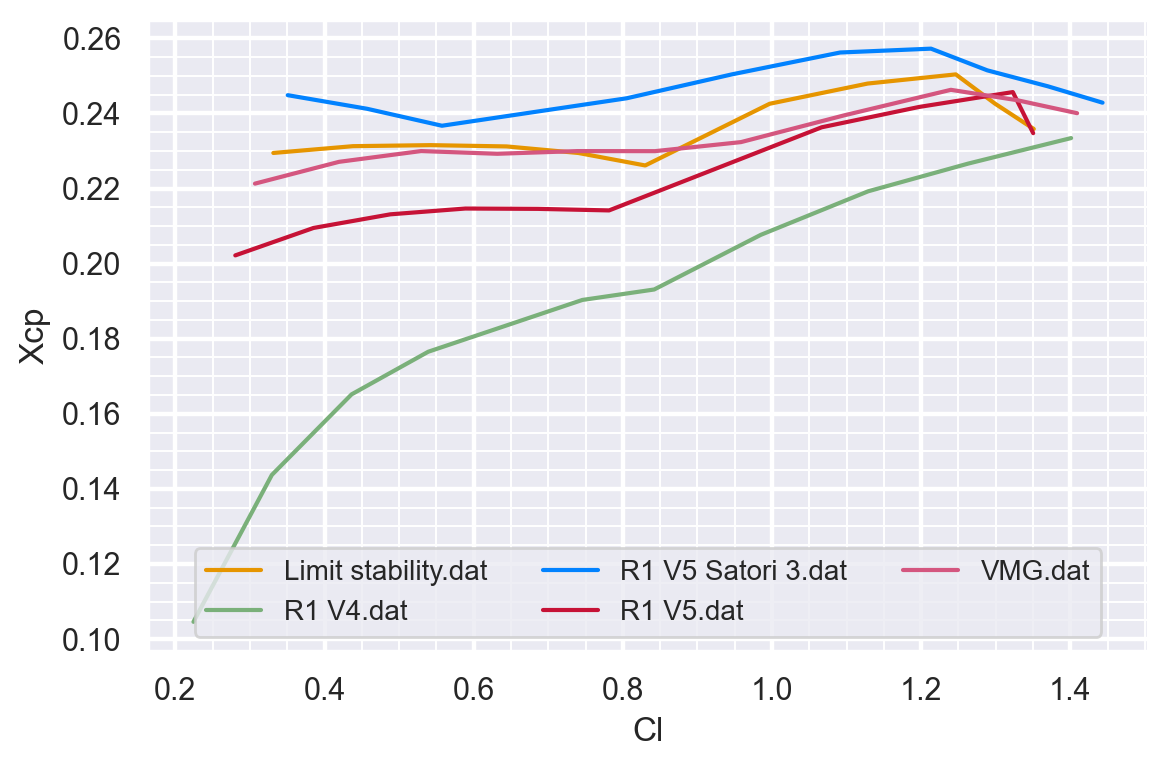
\includegraphics[width=1.0\textwidth]{figures/Stability/airfoils stability.png}
    \caption{$X_{Cp}$ plot against $C_{L}$ }
    \label{fig:X_{Cp} plot against C_{L}}
\end{figure}

It's worth noting that since stability is already noticeable on the beach, when the athlete's speed is at 0 knots, the value of 18 knots (wind speed) serves as a suitable benchmark for comparison with the feedback from the team riders. This is particularly pertinent because when they are stationary on the beach, there are fewer external factors that could affect the results compared to when they are actively riding out at sea.

The figure \ref{fig:X_{Cp} plot against C_{L}} shows that the aerodynamic definition of a kite stability established in \ref{sec:Ch3.1} is in line with the pro kitesurfers' feelings. 

Moreover, the figure \ref{fig:X_{Cp} plot against C_{L}} shows two characteristics that seem to be sources of instability : 
\begin{itemize}
    \item \textbf{high Xcp values}
    \item \textbf{A negative slope of the Xcp curve at low angles of attack}
\end{itemize}

Furthermore, it can be deduced from equation \ref{eq:last equation}, taking into account that for the present kites $X_{A} = 0.07$ and $X_{B} = 0.63$, and considering that $X_{cp} = 0.26$ serves as the stability threshold as depicted in figure \ref{fig:X_{Cp} plot against C_{L}}: \\

\underline{$M_{S} = 1.35$}

%%%%%%%%%%%%%%%%%%%%%%%%%%%%%%%%%%%%%%%%%%%%%%%%%%%%%%%%%%%%%%%%%%%%%%%%%%%%%%%%
%%%%%%%%%%%%%%%%%%%%%%%%%%%%%%%%%%%% SECTION 3 %%%%%%%%%%%%%%%%%%%%%%%%%%%%%%%%%
%%%%%%%%%%%%%%%%%%%%%%%%%%%%%%%%%%%%%%%%%%%%%%%%%%%%%%%%%%%%%%%%%%%%%%%%%%%%%%%%

\section{The add of stability in the airfoil optimization}
\label{sec:Ch3.3}

Taking the stability matter into account, the next step was to generate an optimized airfoil, like in \ref{sec:Ch2.2}, with the add of a stability constraint in the algorithm. 

It is assumed that the more the airfoil is optimized, the more instable it becomes. This is something we can observe on the prototypes we test but also regarding of the figure \ref{fig:X_{Cp} plot against C_{L}}. 

Furthermore, figure \ref{fig:Stability comparison between the existing airfoils and the optimized one} illustrates that the presently optimized airfoil, discussed in Section \ref{sec:Ch2.2}, exhibited excessive instability, making it unsuitable for use in the upcoming prototype.

\begin{figure}[H]
    \centering
    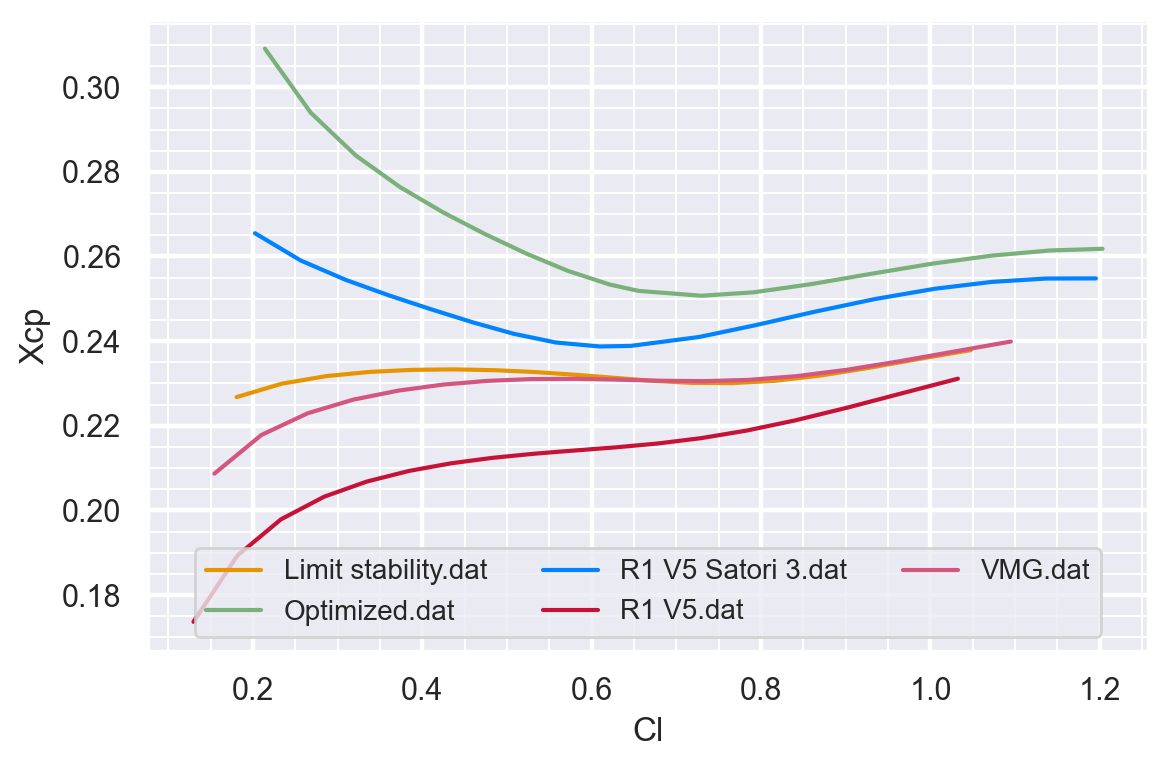
\includegraphics[width=1.0\textwidth]{figures/Stability/optimized airfoil stability.png}
    \caption{Stability comparison between the existing airfoils and the optimized one}
    \label{fig:Stability comparison between the existing airfoils and the optimized one}
\end{figure}

Consequently, the optimization algorithm was adapted to seek an airfoil that lies on the brink of instability while delivering the best possible performance, specifically by maximizing its finesse.

Nonetheless, the Ozone design team opted to delay the adjustment of the value of $M_{S}$, referenced in Section \ref{sec:Ch3.2}, until the team riders had the opportunity to test the optimized airfoil identified in Section \ref{sec:Ch2.2}. Given that the stability constraint imposes significant limitations on the optimization algorithm, it was prudent to first confirm that the current optimized airfoil exhibited instability. However, the team riders have not yet conducted tests on the optimized profile, and the value of $M_{S}$ remains to be verified.

Furthermore, this phase in airfoil design underscored the significance of the initial guess airfoil in the optimization process. It became evident that the algorithm encountered difficulties in reversing the stability graph of an airfoil. In fact, the sign of the slope in the $X_{cp}$ plot at low Cl values would remain unaltered during the optimization process. This implies that starting with an unstable airfoil as the initial guess would not lead to a stable optimized airfoil.
%%%%%%%%%%%%%%%%%%%%%%%%%%%%%%%%%%%% Chapter Template

\chapter{Conclusions} 	% Main chapter title
\label{Conclusion} 		% For referencing the chapter elsewhere, usage \ref{Introduction}

% %%%%%%%%%%%%%%%%%%%%%%%%%%%%%%%%%%%% SECTION 1

% \section{Ozone Kitesurf}
% \label{sec:In1.1}

The primary objective of this internship was to develop Ozone's next-generation R1 formula kite for the 2028 Olympic Games. This endeavor began by utilizing the previous R1 kite version, R1 V4/V5, and the FlySurfer brand's VMG, known for its exceptional performance, as reference points. The overarching goal was to create the most high-performance kite possible for formula kite racing. 
Additionally, this internship aimed to introduce Ozone to a scientific approach to kite design, incorporating aerodynamic coefficients. Understanding the principles governing kite flight and translating these insights into aerodynamic characteristics proved beneficial in the pursuit of a more high-performance kite.

The process commenced with a comparative analysis of existing airfoils. This analysis allowed the experienced design team to discern the specific differences that contributed to the superior performance of the VMG kite compared to the R1 V4/V5. Subsequently, I employed Fluent simulations to meticulously design a new iteration of the R1 kite, resulting in the R1 V5 Satori 3 prototype. This prototype underwent extensive testing by our team riders and demonstrated superior performance compared to the VMG kite.

Furthermore, an optimization algorithm was developed using the Python library Aerosandbox. This algorithm was designed based on the same principles as XFLR5, serving as a preliminary airfoil design tool. It began with the R1 V5 Satori 3 as an initial reference and iteratively converged towards an even higher-performing kite design. Additionally, a 3D optimization algorithm was developed, building upon the principles of the 2D version but incorporating 3D effects and optimizing 3D parameters. While the 3D optimization program has not yet been utilized by Ozone, both algorithms offer valuable tools for the brand's future kite design endeavors.

The 2D optimization program has been employed to design several kites, not limited to the R1 formula kite, which was the focus of this internship. This demonstrates its flexibility in optimizing the parameters as desired by the designer. Furthermore, the 3D optimization program is being utilized by the paraglider design team on their considerably more powerful computers than mine. Should both teams, the paraglider design team and the kitesurf design team, collaborate and utilize this algorithm on their high-performance computers, it has the potential to yield significant benefits for the development of future Ozone kite versions.

In summary, the outcomes of this internship have played a pivotal role in assisting the Ozone team in crafting their next-generation formula kite, the R1 V5, slated for use in the 2028 Olympics. Furthermore, the implementation of optimization algorithms and the calculation of aerodynamic coefficients provide Ozone with a solid foundation for their future kite designs. 

Ultimately, this internship exposed me to the real-world challenges that engineers encounter within a company. The constraints of limited budgets also result in restricted simulation options, and addressing this challenge has encouraged me to explore creative and ingenious solutions. Additionally, the human aspects of water sports, including the sensations experienced by athletes when riding a formula kite, introduced an engineering dimension that I had not previously encountered but proved to be highly beneficial in expanding my open-mindedness.


%\include{chapters/chapter2}		
%\include{chapters/chapter3}	% Uncomment the lines as you write the chapters,
								% where 'chapter3' refers to a file chapter3.tex
%...							% in the 'chapters' folder
								
%\include{chapters/chapter6}

%%%%%%%%%%%%%%%%%%%%%%%%%%%%%%%%%%%%%%%%%%%%%%%%%%%%%%%%%%%%%%%%%%%%%%%%%%%%%%%%%%%%%%%%%
% Print the bibliographic references using the ieeetr format from the 'sampleRefs.bib' file (root folder)

% \clearpage

\addcontentsline{toc}{chapter}{References}
\bibliographystyle{plain} % We choose the "plain" reference style
\bibliography{references} % Entries are in the refs.bib file

								% a good option to make bib files is https://www.jabref.org/
			
%%%%%%%%%%%%%%%%%%%%%%%%%%%%%%%%%%%%%%%%%%%%%%%%%%%%%%%%%%%%%%%%%%%%%%%%%%%%%%%%%%%%%%%%%
%\begin{appendices}
% Include the appendices of the document as separate files from the 'chapters' folder

%% Appendix A

\chapter{Título do Anexo} % Main appendix title
\label{AppendixA} % For referencing this appendix elsewhere, use \ref{AppendixA}

%%%%%%%%%%%%%%%%%%%%%%%%%%%%%%%%%%%%%%%%%%%%%%%%%%%%%%%%%%%%%%%%%%%%%%%%%%%%%%%%%%
\section{Secção}

\lipsum[1]

%%%%%%%%%%%%%%%%%%%%%%%%%%%%%%%%%%%%%%%%%%%%%%%%%%%%%%%%%%%%%%%%%%%%%%%%%%%%%%%%%%
\section{Mais uma secção do Anexo~\ref{AppendixA}}

\lipsum[1]

	% Uncomment the lines as you write the appendices,
%\include{chapters/appendixB}	% or comment the lines if not used

%\end{appendices}
%%%%%%%%%%%%%%%%%%%%%%%%%%%%%%%%%%%%%%%%%%%%%%%%%%%%%%%%%%%%%%%%%%%%%%%%%%%%%%%%%%%%%%%%%
\end{document}  
